\chapter{Aggregate Land Development (ALD) Module}

In each simulation year, the Aggregate Land Development (ALD) module produces a floorspace inventory based on ALD annual increments and decrements of floorspace by category and alpha zone from:
\begin{itemize}
\item Total budgeted Dollar-value amounts of residential and nonresidential construction produced by the NED Module for the simulation year (construction\_forecast.csv), and
\item Inventories of floorspace by category and alpha zone for the previous simulation year (ActivityLocations.csv from previous year).
\end{itemize}

\noindent The module works at two levels of spatial aggregation. Dollar-value construction amounts and decrease amounts (due to demolition and conversion) are allocated among 15 regions. (Land development markets tend to be regional in scope.)  All subsequent allocations to floorspace categories and alpha zones are done by region.

ALD's allocation processes use information from several sources:
\begin{itemize}
\item Residential and non-residential activity quantities from the AA module (allocation to regions)
\item Floorspace occupancy rates from the AA module (allocation to space types within regions)
\item Floorspace prices from the AA module (allocation to zones)
\item Land area by comprehensive plan category and alpha zone as a model scenario input. (capacity used in allocation to zones)
\end{itemize}

\section{Theoretical Basis}
The ALD module determines the changes in floorspace by type in each alpha zone in each simulation year based on residential and non-residential construction forecasts (NED), floorspace prices and vacancies (AA), floorspace quantities (ALD), and the availability of land by current zoning and comprehensive plan designation. It does this using a series of connected logit and Cobb-Douglas allocation models.

The change in floorspace for a model simulation year are based on the total dollar-value quantities of residential and non-residential floorspace construction determined for the year for the entire model area by the NED Module. These construction amounts include construction that replaces existing floorspace (lost though demolition or conversion) as well as construction of new floorspace on vacant land. The net change in floorspace is therefore the total value of floorspace constructed (from NED) minus the value of floorspace removed. The value of the floorspace removed is calculated as a fixed proportion of the value of floorspace constructed based on comparison of NED calibration data and net floorspace change calculated from FW Dodge data. ALD allocates the floorspace declines and increases separately rather than allocating the net change in order to better represent responses in the floorspace market to changing activity patterns over time.

The floorspace increase and decrease quantities are first allocated among 15 regions. All subsequent allocation to floorspace types and alpha zones is done within each region. The rationale for this approach is that markets for floorspace development tend to have a regional orientation, rather than a statewide or larger orientation. The regions used by the ALD module are collections of counties located near each other that tend to have close linkages with one another and/or share a similar geographic relationship to other regions. The regions were determined using  expert judgment in a manor similar to how beta zone groupings were formed from alpha zones, or how aggregate district area are formed from TAZs in travel demand models. 

The residential and non-residential increases and decreases are allocated using Cobb-Douglas production functions where the inputs are the proportion of total activity in each region and the proportion of total activity change in each region. The form of these functions is the same for all residential and non-residential increase and decrease models, but with four different sets of estimated parameters (residential increase, non-residential increase, residential decrease, non-residential decrease). 

After the dollar values of residential and non-residential floorspace increases and decreases have been allocated to regions, all subsequent steps are carried out on a regional basis. First, the residential and non-residential increases and decreases are split into the floorspace categories. This is done using logit models where the input variables are previous proportions of space by category and vacancy rates by category. Once the dollar values are split by category, they are converted into space (sqft) quantities using exogenously-specified construction cost rates. 

Next, the floorspace increases and decreases of each type are allocated to alpha zones. Floorspace decreases are allocated using a Cobb-Douglas production function where the input variables are the existing proportion of that type of floorspace in each zone and the price determined by the AA module for that type of floorspace in the corresponding beta zone. Floorspace increases are allocated among the alpha zones also using a Cobb-Douglas formula. In this case, the inputs to the function are the existing proportion of that type of floorspace in each zone, the price determined by the AA module for that type of floorspace in the corresponding beta zone and the capacity of each alpha zone to accommodate additional floorspace of the type. Floorspace capacity is a function of how much land is planned for development by generalized zoning category, the compatibility of each floorspace category with each plan category and the allowable floor area ratio for each floorspace category in each plan category.

\section{Quantity Definitions and Categories}
ALD makes development changes at the alpha zone level, although initial allocation of space utilizes a set of 15 regions representing land development markets, previously shown in Figure \ref{fig:ald-regions} (page \pageref{fig:ald-regions}). AA output data used as inputs to ALD is provided at the beta zone level.

ALD uses categories of floorspace listed previously in Table \ref{tab:floorspace-categories} (page \pageref{tab:floorspace-categories}). Zoning categories are identified in Table \ref{tab:ald_zoning_cat}. The set of zoning codes used in ALD were adopted from the Department of Land Conservation and Development's generalized zoning codes, which aggregated all the local jurisdictional zoning codes from the approximately 300 jurisdictions across Oregon into 55 generalized zoning categories. Data describing the allowed floorspace types and intensities are discussed with zoning inputs in \S\ref{sec:ald-zoning-data}. 

\begin{sidewaystable}
\centering
\caption{ALD zoning categories (inputs/parameters/zoning\_definitions.csv)}\label{tab:ald_zoning_cat}
\begin{tabular}{ccl|ccl}
\hline
Code & Name & Zoning description & Code & Name & Zoning description \\
\hline
1 & VLDR & Very Low-density residential & 28 & EFU80 & Exclusive Farm Use 80~~~~~~~~~~~~~~~~~~~~~~~~~~~~~~~ \\
\gray 2 & LDR & Low-density residential & 29 & EFU160 & Exclusive Farm Use 160+ \\
3 & MLDR & Medium Low-density residential & 30 & FF20 & Mixed Farm-Forest 20 \\
\gray 4 & MDR & Medium-density residential & 31 & FF40 & Mixed Farm-Forest 40 \\
5 & MHDR & Medium High-density residential & 32 & FF80 & Mixed Farm-Forest 80 \\
\gray 6 & HDR & High-density residential & 33 & FF160 & Mixed Farm-Forest 160+ \\
7 & VHDR & Very High-density residential & 34 & SF80 & Secondary Forest 80 \\
\gray 8 & MURL & Mixed use commercial and residential low & 35 & PF80 & Prime Forest 80 \\
9 & MURM & Mixed use commercial and residential medium & 36 & RR10 & Rural Residential 10 acres \\
\gray 10 & MURMH & Mixed use commercial and residential med-high & 37 & RR5 & Rural Residential 5 acres \\
11 & MURH & Mixed use commercial and residential high & 38 & RR2 & Rural Residential 2-4 acres \\
\gray 12 & MURVH & Mixed use commercial and residential v.high & 39 & RR1 & Rural Residential 1 acre \\
13 & MUREH & Mixed use commercial and residential extremely high & 40 & RC & Rural Commercial \\
\gray 14 & CC & Commercial - Central & 41 & UCRC & UC Rural Commercial \\
15 & CG & Commercial - General & 42 & RI & Rural Industrial \\
\gray 16 & CN & Commercial - Neighborhood & 43 & UCRI & UC Rural Industrial \\
17 & CO & Commercial - Office & 44 & OSC & Open Space/Conservation \\
\gray 18 & PF & Public and semi-public uses & 45 & MA & Mineral and Aggregate \\
19 & POS & Parks and open space & 46 & CE & Coastal Estuarine \\
\gray 20 & IC & Industrial Campus & 47 & CS & Coastal Shorelands \\
21 & IO & Industrial Office & 48 & BD & Beaches and Dunes \\
\gray 22 & IL & Light industrial & 49 & RNG & Federal Range \\
23 & IH & Heavy industrial & 50 & FOR & Federal Forest \\
\gray 24 & FUD & Future urban development & 51 & IRM & Indian reservation/tribal trust \\
25 & MFL10 & Marginal Farm Land 10+ & 52 & CEE & Combo equal emphasis \\
\gray 26 & EFU20 & Exclusive Farm Use 20+ & 53 & CPE & Combo with priority emphasis \\
27 & EFU40 & Exclusive Farm Use 40+ & 54 & O & Other \\
\hline
\end{tabular}
\end{sidewaystable}

\section{Component Models}\label{sec:aa-component-models}
The objective of the ALD module is to identify where modelwide construction dollars (in 2009 dollars) from the NED module will be spent and in what type of development. The component models are as follows. Except as noted, each model step below has a residential model and a corresponding non-residential model. A flowchart of the ALD model is shown in Figure \ref{fig:ald-components}, and includes the following functionality:

\begin{figure}
\centering
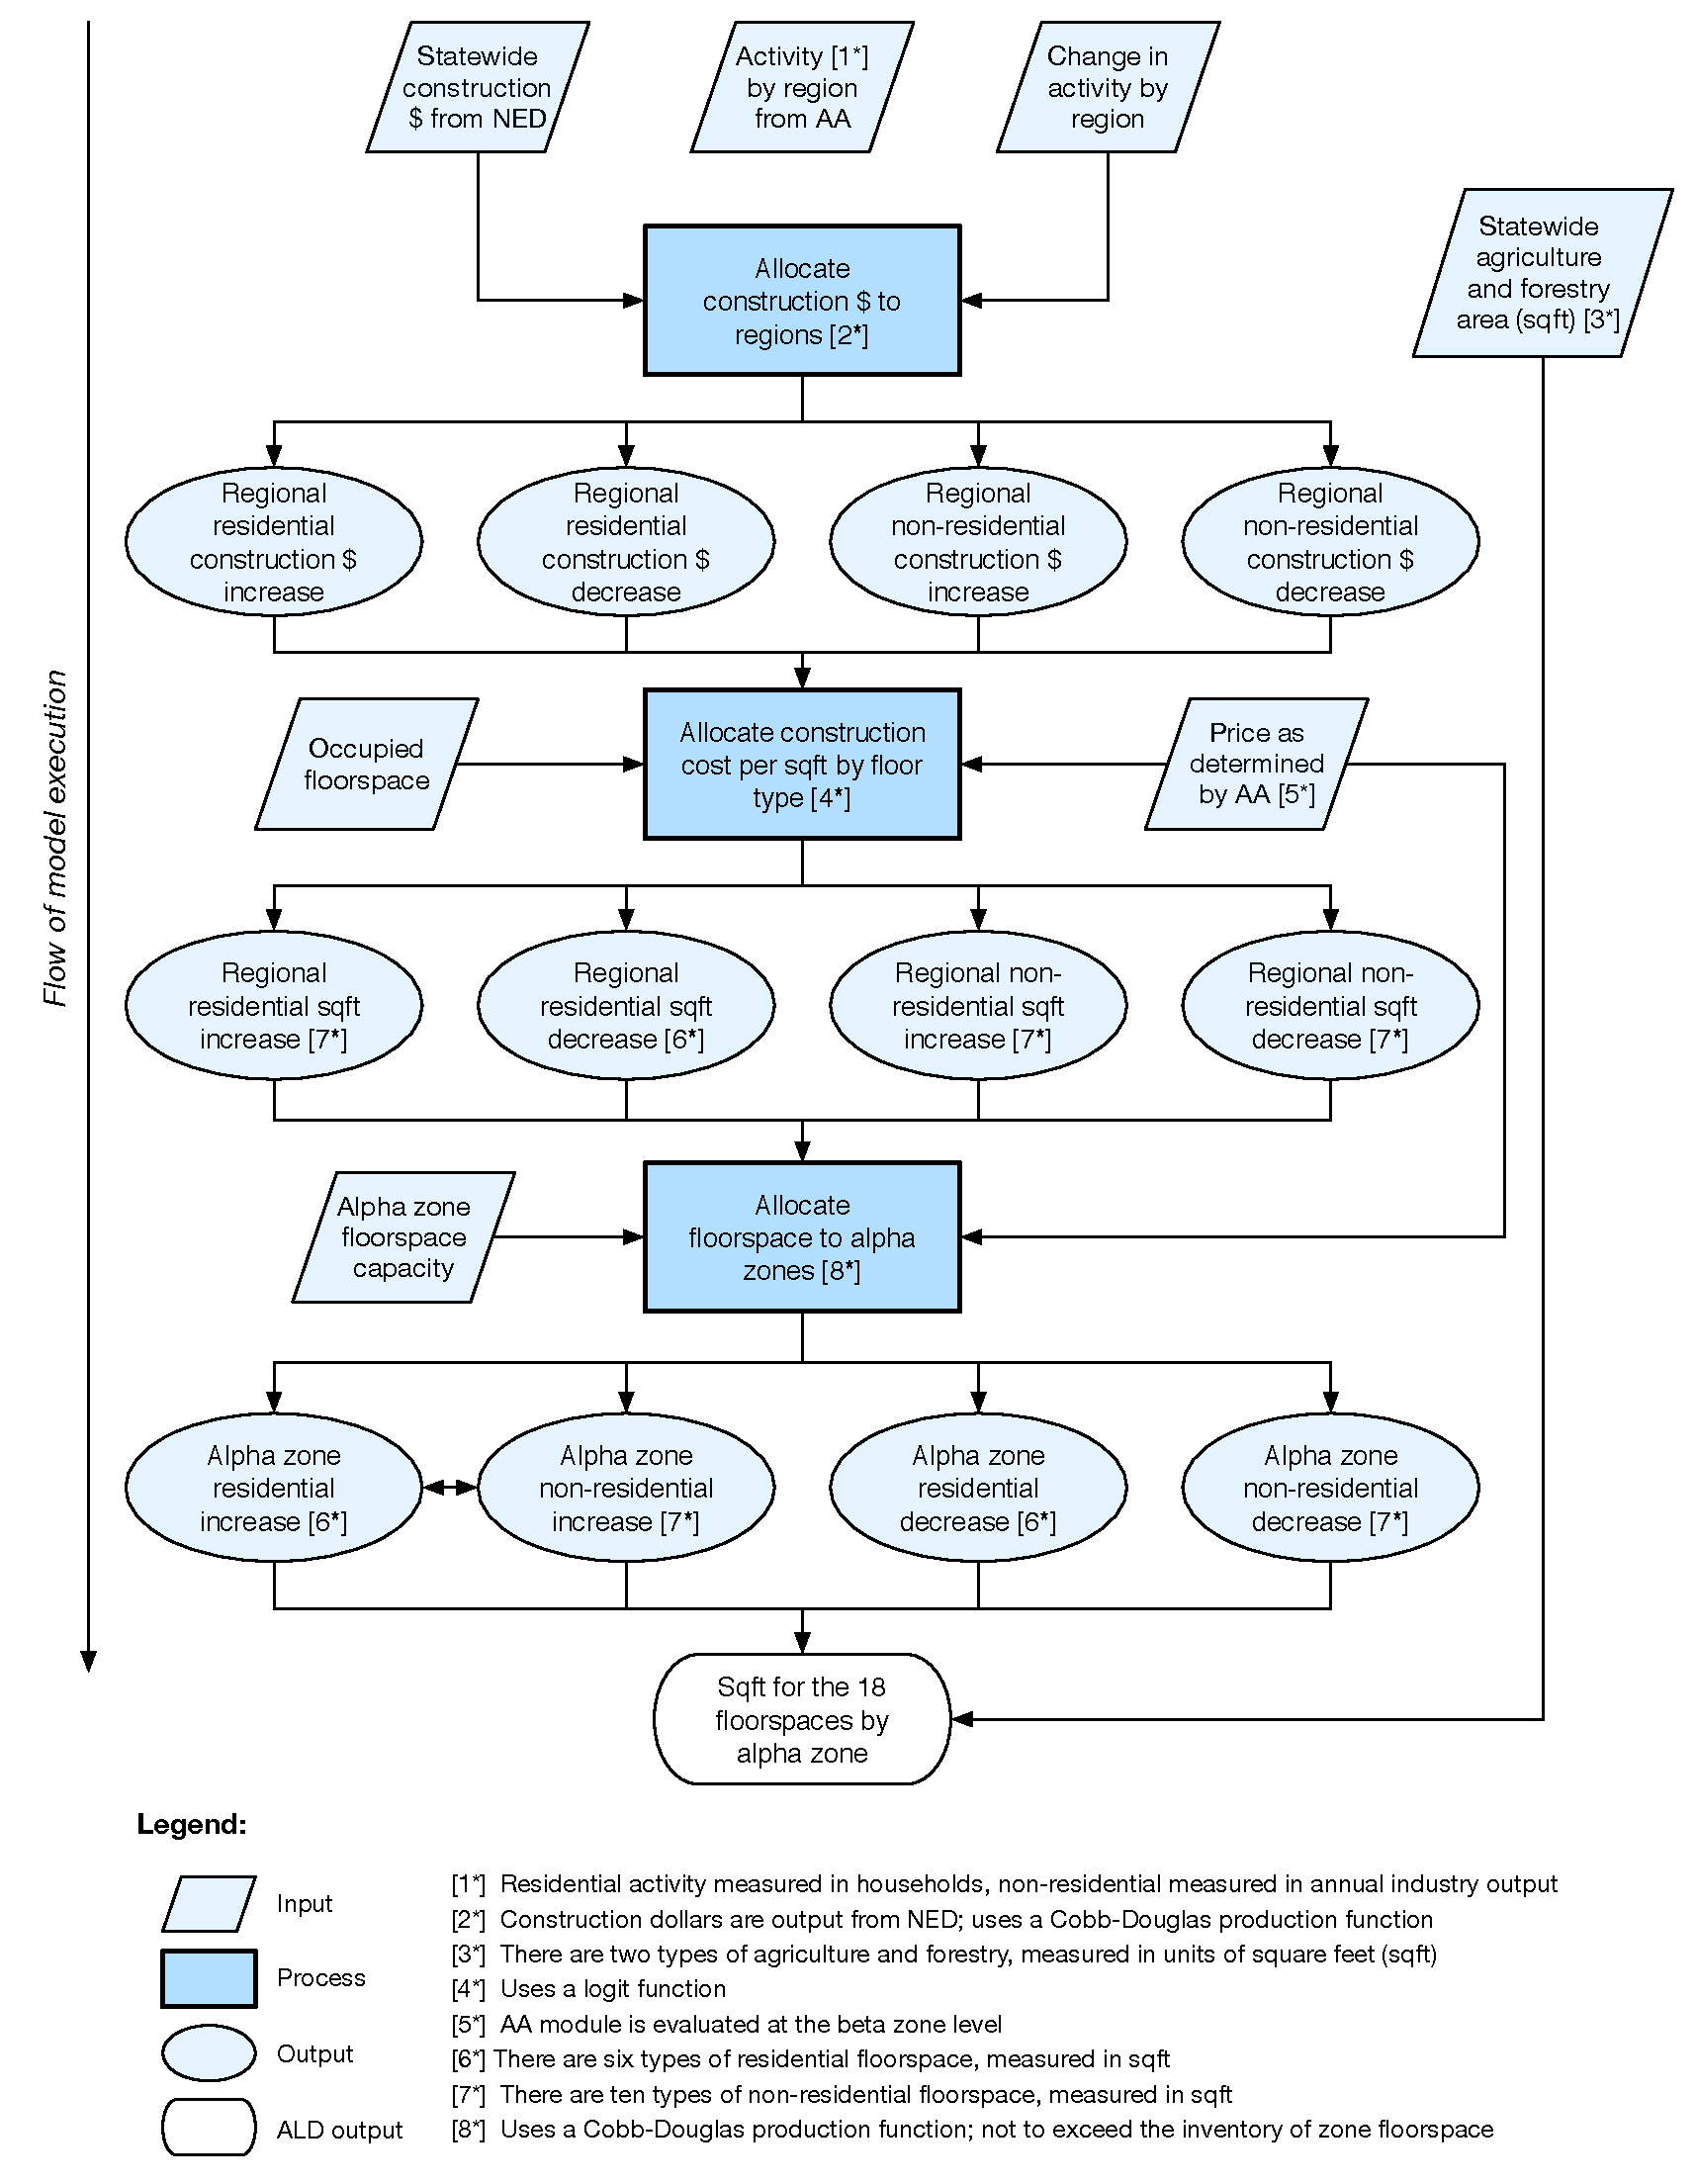
\includegraphics[width=6.5in]{ald/ald-alt-flowchart}
\caption{ALD model components flowchart}\label{fig:ald-components}
\end{figure}

\begin{itemize}
\item \textit{Total model-wide dollar values of residential and non-residential floorspace construction are allocated among 15 regions in the model area.} All subsequent allocations among floorspace types and alpha zones are done within each region. Construction dollars are allocated among regions using a Cobb-Douglas formulation where the independent variables are the region proportions of total activity in the previous year and the region proportions of the change in total activity over the previous two years. The model also incorporates region-specific constants. This process is described in more detail in \S\ref{sec:ald-step1}.
\item \textit{Total model-wide decreases in residential and non-residential floorspace (due to demolition or conversion) are estimated and allocated among regions.} The model-wide value of the floorspace demolished or converted is calculated as a fixed proportion of the model-wide value of floorspace constructed. The model-wide decreases are allocated among regions using the same form of Cobb-Douglas production function as used to allocate the construction increases. Region-specific constants are also included. This process is described in more detail in \S\ref{sec:ald-step1}.
\item \textit{The regional increase values are allocated to floorspace categories} using a logit model where the utility is a function of vacancy rates and the previous quantities of floorspace by category. The model includes alternative specific constants for each floorspace type in each region. The allocated construction values by floorspace category are converted to floorspace area increases (square feet) using model-wide average floorspace construction costs. This process is described in more detail in \S\ref{sec:ald-step2}.
\item \textit{The regional floorspace decrease values are allocated to floorspace categories} using a logit model having the same form as the model for allocating regional increase values. The model includes alternative specific constants for each floorspace type in each region. Floorspace value decreases are converted into area measures (square feet) using the model-wide average floorspace construction costs since the decrease values represent the value of the space lost and not the cost of demolition or conversion. This process is described in more detail in \S\ref{sec:ald-step2}.
\item \textit{The regional floorspace decreases by floorspace category are allocated to alpha zones} using a Cobb-Douglas production function where the input variables are the proportion of total regional floorspace of the category in each zone and the price determined by the AA module for that type of floorspace in the corresponding beta zone. The decrease in floorspace in any zone is not allowed to exceed the inventory of floorspace in the zone. This process is described in more detail in \S\ref{sec:ald-step3}.
\item To allocate the region floorspace increases in each category to alpha zones it is necessary to calculate the capacity of each alpha zone for accommodating floorspace of each category. Floorspace capacity is a function of how much land is currently zoned or planned for development by zoning category, the compatibility of each floorspace category with each plan category and the allowable floor area ratio for each floorspace category in each plan category. A logit model is used to set initial proportions of land by zoning category to floorspace categories. Those initial proportions are then balanced to current floorspace demand by alpha zone while adhering to input development constrains of what floorspace types can and cannot be allocated to a given zoning category quantity. Floor area ratios are also used in the balancing process, as the balancing process must convert between land area and floorspace area, floorspace area capacity being what is ultimately used in allocation of floorspace increases by alpha zone and available land area by zoning category being what is input to the model at the alpha zone level. This process is described in more detail in \S\ref{sec:ald-step4}.
\item \textit{Floorspace increases for each region and category are allocated to alpha zones} using a Cobb-Douglas production function where the inputs are the proportion of total regional floorspace of the category in each zone, the price determined by the AA module for that type of floorspace in the corresponding beta zone and the floorspace capacity for the category in each zone. This process is described in more detail in \S\ref{sec:ald-step5}.
\end{itemize}

\subsection{Allocation of Modelwide Construction Dollars into Regional Dollar Value Increases and Decreases}\label{sec:ald-step1}  % 5.3.1
The first function of ALD is to separately allocate dollar-value production of residential and non-residential construction from the NED module for the entire model area among 15 regions in the model area. In addition, since the total value of construction in the entire model area includes the replacement of floorspace that is removed somewhere in the model area as well as net new floorspace, it is necessary to calculate the value of residential and non-residential floorspace decreases and allocate them to the regions as well. 

Construction dollars are allocated among regions using a Cobb-Douglas model where the independent variables are the region proportions of total activity in the previous year and the region proportions of the change in total activity over the previous two years. The equation has the form:
\begin{equation}\label{eq:5.01}  % 5.01
NIVQ_r = NIVQ \cdot \left( CD_r / \sum_r{CD_r} \right)
\end{equation}

\noindent with:
\begin{equation}\label{eq:5.02}   % 5.02
CD_r = (ActProp_r + \beta_{1v})^{\beta_{2v}} \cdot (ActChgProp_r + \beta_{3v})^{\beta_{4v}} \cdot A_{scr}
\end{equation}

\noindent where:
\begin{align*}
NIVQ &= \text{modelwide total residential (nonresidential) construction value by year from NED} \\
 &~~~~~\text{(construction\_forecast.csv)} \\
NIVQ_r &= \text{residential (nonresidential) construction value for region $r$} \\
CD_r &= \text{Cobb-Douglas production function for region $r$ (estimated)} \\
ActProp_r &= \text{proportion of total modelwide residential (nonresidential) activity occurring in} \\
 &~~~~~\text{region $r$ (see notes below)} \\
ActChgProp_r &= \text{proportion of total modelwide residential (nonresidential) activity change} \\
 &~~~~~\text{occurring in region $r$ (see notes below)} \\
\beta_{*v} &= \text{coefficients estimated separately for residential and nonresidential construction} \\
 &~~~~~\text{(estimated)} \\
Asc_r &= \text{alternative specific constant for region estimated separately for residential} \\
 &~~~~~\text{and nonresidential construction (adjusted)}
\end{align*}

\noindent Decreases in the value of floorspace are calculated from the modelwide construction total are allocated to regions as follows:
\begin{equation}\label{eq:5.03}  % 5.03
NDVQ_r = D_f \cdot NIVQ \cdot \left( CD_r / \sum_r{CD_r} \right)
\end{equation}

\noindent with:
\begin{equation}  % 5.04
CD_r = (ActProp_r + \beta_{5v})^{\beta_{6v}} \cdot (ActChgProp_r + \beta_{7v})^{\beta_{8v}} \cdot A_{scr}
\end{equation}

\noindent where $D_f$ modelwide proportion of residential (nonresidential) floorspace construction value, and the other variables are defined as described above.

The measure of activity used to calculate the proportions of total activity and the proportions of activity change is measured using the ``quantity'' output from the AA module. This is households, in the case of residential activities and annual output in 2009 dollars, in the case of non-residential activities (from AA ExchangeResults.csv prior year output aggregated to ALD regions).

The proportion of activity change is calculated after the regional activity change values are rescaled by subtracting the minimum regional value from all regional values. The rescaling is necessary to assure that the activity change proportions are in the range of 0 to 1. For the first two simulation years, when there is no computable activity change, it is assumed that all regions have an equal proportion of the activity change.


\subsection{Allocation of Regional Dollar Increases and Decreases into Floorspace Types}\label{sec:ald-step2}   % 5.3.2
Regional residential and non-residential floorspace construction and decreases are allocated separately to the floorspace categories using a logit model with utility functions that include regional vacancy rates by floorspace category and proportions of previous year floorspace value in each floorspace category. In calibration, the second term in equation \ref{eq:5.06} was modified from the construction cost value, to the AA value (based on prior year AA floorspace prices). Thus, this term serves not only as a size measure, but also as a signal for which floorspace types are in demand (indicated by higher prices), which helps to allocate construction dollars more effectively. The logit model for floorspace construction has the form:
\begin{equation}\label{eq:5.05}   % 5.05
NIVQ_{f,r} = NIVQ_r \cdot exp(\lambda_{q1} \cdot U_{f,r}) / \sum_f exp(\lambda_{q1} \cdot U_{f,r})
\end{equation}
\noindent with:
\begin{equation}  % 5.06
U_{f,r} = {\beta_{q1,f}} \cdot VacRate_{f,r} + {\beta_{q2}} \cdot ln \left( TVQ_{f,r} / \sum_f TVQ_{f,r} \right) + ASC_{f,r}
\label{eq:5.06}
\end{equation}

\noindent where:
\begin{align*}
NIVQ_{f,r} &= \text{value of floorspace construction allocated to category $f$ in region $r$} \\
NIVQ_r &= \text{total value of floorspace construction in region $r$ (equation \ref{eq:5.01})} \\
U_{f,r} &= \text{utility of floorspace category $f$ in region $r$} \\
\lambda_{q1} &= \text{dispersion parameter of the logit model (estimated separately for residential} \\
 &~~~~~\text{and non-residential floorspace construction)} \\
VacRate_{f,r} &= \text{average vacancy rate for floorspace category $f$ in region $r$ in the} \\
 &~~~~~\text{previous year (calculated from AA ExchangeResults.csv occupied space use and} \\
 &~~~~~\text{ALD FloorspaceInventory.csv total space inventory)} \\
TVQ_{f,r} &= \text{dollar value of floorspace category $f$ in region $r$ in the previous year} \\
 &~~~~~\text{(calculated from ALD FloorspaceInventory.csv floorspace inventory and} \\
 &~~~~~\text{AA ExchangeResults.csv module square foot values of floorspace summed to} \\
 &~~~~~\text{floorspace category)} \\
\beta_{q1,f} &= \text{coefficient estimated separately for residential and non-residential} \\
 &~~~~~\text{construction (estimated)} \\
\beta_{q2} &= \text{sensitivity coefficient for the previous year zone proportion of total} \\
 &~~~~~\text{floorspace of this type (estimated)} \\
ASC_{f,r} &= \text{alternative specific constant for construction of floorspace category $f$ in} \\
 &~~~~~\text{region $r$ (estimated)}
\end{align*}

\noindent The logit model for floorspace decreases has the form:
\begin{equation}\label{eq:5.07}   % 5.07
NDVQ_{f,r} = NDVQ_r \cdot a \left[ exp({\lambda_{q2}} \cdot U_{f,r}) / \sum_f exp({\lambda_q} \cdot U_{f,r}) \right]
\end{equation}
\noindent with:
\begin{equation}   % 5.08
U_{f,r} = {\beta_{q3,f}} \cdot VacRate_{f,r} + \beta_{q4} \cdot ln \left( TVQ_{f,r} / \sum_f TVQ_{f,r} \right) + ASC_{f,r}
\end{equation}

\noindent where:
\allowdisplaybreaks
\begin{align*}
NDVQ_{f,r} &= \text{value of floorspace decrease allocated to category $f$ in region $r$} \\
NDVQ_r &= \text{total value of floorspace decrease in region (equation \ref{eq:5.03})} \\
U_{f,r} &= \text{utility of floorspace category $f$ in region $r$} \\
\beta_{q2} &= \text{dispersion parameter of the logit model estimated separately for residential} \\
 &~~~~~\text{and non-residential floorspace construction (estimated)} \\
VacRate_{f,r} &= \text{average vacancy rate for floorspace category $f$ in region $r$ in the previous} \\
 &~~~~~\text{year (calculated from AA ExchangeResults.csv occupied space use and ALD} \\
 &~~~~~\text{FloorspaceInventory.csv total space inventory)} \\
TVQ_{f,r} &= \text{dollar value of floorspace category $f$ in region $r$ in previous year (calculated from} \\
 &~~~~~\text{ALD FloorspaceInventory.csv floorspace inventory and AA ExchangeResults.csv} \\
 &~~~~~\text{square foot values of floorspace summed to floorspace category)} \\
\beta_{q3,f} &= \text{coefficient estimated separately for residential and non-residential construction} \\
 &~~~~~\text{(estimated)} \\
\beta_{q4} &= \text{sensitivity coefficient for the previous year zone proportion of total floorspace} \\
 &~~~~~\text{of this type (estimated)} \\
ASC_{f,r} &= \text{alternative specific constant for decrease in floorspace category $f$ in region $r$} \\
 &~~~~~\text{(estimated)}
\end{align*}

\noindent The regional average vacancy rate for a given category of floorspace is calculated as follows:
\begin{equation}   % 5.09
VacancyRate_{f,r} = \left( \sum_{\alpha,r} PrevQ_{f,\alpha,r} - \sum_{\beta,r} Occupied_{f,\beta,r} \right) / \sum_{\alpha,r} PrevQ_{f,\alpha,r}
\end{equation}

\noindent where:
\begin{align*}
\alpha &= \text{index representing alpha zones in region $r$} \\
\beta &= \text{index representing betazones in region $r$} \\
PrevQ_{f,\alpha,r} &= \text{building area-based quantity of total floorspace of category $f$ in zone $\alpha$} \\
 &~~~~~\text{of region $r$ in the previous year (ALD previous year FloorspaceInventory.csv by} \\
 &~~~~~\text{alpha zone)} \\
Occupied_{f,\beta,r} &= \text{building area-based quantity of occupied floorspace of category $f$ in zone} \\
 &~~~~~\text{$\beta$ of region $r$ in the previous year (AA ExchangeResults.csv by beta zone)}
\end{align*}

The dollar-value quantity of floorspace in each category $f$ in each region is converted into an equivalent area-based quantity (in building sqft) using modelwide average unit construction costs (per building sqft) specified exogenously. It is calculated as follows:
\begin{equation}\label{eq:5.10}  % 5.10
NIQ_{f,r} = NIVQ_{f,r} / ConstrCost_f
\end{equation}
\begin{equation}\label{eq:5.11}  % 5.11
NDQ_{f,r} = NDVQ_{f,r} / ConstrCost_f
\end{equation}

\noindent where:
\begin{align*}
NIQ_{f,r} &= \text{building area-based quantity of floorspace construction allocated to category $f$ in} \\
 &~~~~~\text{region $r$} \\
NIVQ_{f,r} &= \text{value of floorspace construction allocated to category $f$ in region $r$ (equation \ref{eq:5.05})} \\
NDQ_{f,r} &= \text{building area-based quantity of floorspace decrease allocated to category $f$ in} \\
 &~~~~~\text{region $r$} \\
NDVQ_{f,r} &= \text{value of floorspace decrease allocated to category $f$ in region $r$ (equation \ref{eq:5.07})} \\
ConstrCost_f &= \text{modelwide average unit construction costs for floorspace category $f$ (exogenous} \\
 &~~~~~\text{ConstructionCosts.csv)}
\end{align*}

\subsection{Allocation of Zonal Floorspace Decrease}\label{sec:ald-step3}   % 5.3.3
Regional decreases in the quantity of floorspace in each category are allocated among alpha zones in each region using a Cobb-Douglas model where the input variables are the proportion of total regional floorspace of the category in each zone and the price determined by the AA module for that type of floorspace in the corresponding beta zone. The equations for this model are as follows:
\begin{equation}\label{eq:5.12}  % 5.12
DQ_{f,\alpha,r} = NDQ_{f,r} \cdot (CD_{f,\alpha,r}) / \sum_\alpha{CD_{f,\alpha,r}}
\end{equation}

\noindent with:
\begin{equation}   % 5.13
CD_{f,\alpha,r} = (PrevProp_{f,\alpha,r})^{\beta_{3f}} \cdot (Price_{f,\alpha,r})^{\beta_{4f}}
\end{equation}
\noindent where:
\begin{align*}
\alpha &= \text{index representing a specific alpha zone} \\
DQ_{f,\alpha,r} &= \text{decrease in quantity of floorspace category $f$ in alpha zone $\alpha$ in region $r$} \\
NDQ_{f,r} &= \text{building area-based quantity of floorspace decrease allocated to category $f$ in} \\
 &~~~~~\text{region $r$ (equation \ref{eq:5.11})} \\
CD_{f,\alpha,r} &= \text{Cobb-Douglas production function for floorspace category $f$ in alpha zone $\alpha$} \\
 &~~~~~\text{in region $r$ (estimated)} \\
PrevProp_{f,\alpha,r} &= \text{share of previous year regional floorspace quantity of category $f$ in alpha} \\
 &~~~~~\text{zone $\alpha$ (using ALD previous year FloorspaceInventory.csv)} \\
Price_{f,\alpha,r} &= \text{previous year price of floorspace quantity of category $f$ in the beta zone in} \\
 &~~~~~\text{which alpha zone $\alpha$ is located (previous year AA ExchangeResults.csv)} \\
\beta_{3f}, \beta_{4f} &= \text{allocation coefficients (estimated separately for residential and non-residential} \\
 &~~~~~\text{decreases)}
\end{align*}

\subsection{Land Capacity Calculation}\label{sec:ald-step4}   % 5.3.4
To allocate the region floorspace increases in each category to alpha zones it is first necessary to calculate the capacity of each alpha zone for accommodating floorspace of each category. Floorspace capacity is a function of how much land is currently zoned or planned for development by plan category, the compatibility of each floorspace category with each zoning category and the allowable floor area ratio for each floorspace category in each zoning category. The following logit model is used to set initial proportions of land by zoning category to floorspace categories:
\begin{equation}\label{eq:5.14}   % 5.14
LandProp_{f,z} = exp(U_{f,z}) / \sum_f exp(U_{f,z})
\end{equation}
\noindent with:
\begin{equation}\label{eq:5.15}   % 5.15
U_{f,z} = \lambda_p \left[ stc \cdot ln(LandSQFT_f) + ln(Compat_{f,z}) \right]
\end{equation}
\noindent subject to the constraint $exp(U_{f,z}) \ge 0$, and where:
\begin{align*}
LandProp_{f,z} &= \text{proportion of zoning category $z$ land area allocated to floorspace type $f$} \\
U_{f,z} &= \text{utility of allocating land in zoning code $z$ to floorspace type $f$} \\
Compat_{f,z} &= \text{compatibility of floorspace type $f$ in zoning category $z$ (exogenous,} \\
 &~~~~~\text{zoning\_compatibility.csv)} \\
stc &= \text{parameter for the sensitivity to the size term (estimated)} \\
\lambda_{p} &= \text{dispersion parameter for the sensitivity to input compatibility matrix (estimated)} \\
LandSQFT_f &= \text{baseyear modelwide land area devoted to each floorspace type (exogenous,} \\
 &~~~~~\text{LandSQFTxFLR.csv, which comes from inputs stored in Visum, SI)}
\end{align*}

The land area capacities for each floorspace category in each alpha zone are initially calculated from the proportional allocation of zoning categories to floorspace categories, the inventory of zoning by type and alpha zone and maximum floor area ratios by zoning type and floorspace category as follows:
\begin{equation}\label{eq:5.16}    % 5.16
LandCap_{z,f,\alpha} = LandProp_{f,z} \cdot ZoneArea_{z,\alpha}
\end{equation}
\noindent where:
\begin{align*}
LandCap_{z,f,\alpha} &= \text{land area capacity for zoning category and floorspace category $f$ in alpha zone $\alpha$} \\
LandProp_{f,z} &= \text{proportion of zoning category $z$ land area allocated to floorspace type $f$} \\
 &~~~~~\text{(equation \ref{eq:5.14})} \\
ZoneArea_{z,\alpha} &= \text{land area with zoning category $z$ in alpha zone $\alpha$ (exogenous,} \\
 &~~~~~\text{LandSQFTxZoning.csv, which is output from inputs stored in Visum, SI)}
\end{align*}

The initial land area capacities calculated in equation \ref{eq:5.15} are informed by zoning compatibility, but not by demand. These initial capacities, for example, may create a 50/50 capacity split of warehouse and light industrial for a given zone, but in this example the zoning allows for the area to be one hundred percent filled with either light industrial or warehouse. Without adjusting to demand, the given zone might have a demand for ten percent light industrial and ninety percent warehouse, but because the 50/50 split has been set to capacity the development of warehouse space in that area would be artificially constrained.  

Therefore, a multi-dimensional balancing method is applied that respects the hard constraints of total land capacity by alpha zone, zoning compatibility between zoning category and floorspace categories, and total buildable floorspace by alpha zone. The balancing process starts with the initial land area capacities calculated in equation \ref{eq:5.16} as the initial seed to be balanced. The land square footage across zoning and floorspace categories are summed to alpha zone to create a total buildable land area by alpha zone.  Next initial floorspace capacity proportions are calculated by multiplying the land area capacities calculated in equation \ref{eq:5.16} by the maximum floor area ratios by zoning type and floorspace category as follows:
\begin{equation}\label{eq:5.17}    % 5.17
FloorProp_{z,f,\alpha} = FloorCap_{z,f,\alpha} / \sum_{z,f} FloorCap_{z,f,\alpha}
\end{equation}
\noindent with: 
\begin{equation}    % 5.18
FloorCap_{z,f,\alpha} = LandCap_{z,f,\alpha} \cdot FAR_{f,z}
\end{equation}
\noindent where:
\begin{align*}
FloorProp_{z,f,\alpha} &= \text{proportion of available floorspace for each zoning category in alpha zone $\alpha$} \\
 &~~~~~\text{and floorspace category $f$} \\
FloorCap_{z,f,\alpha} &= \text{floorspace capacity for zoning category and floorspace category $f$ in alpha} \\
 &~~~~~\text{zone $\alpha$} \\
LandCap_{z,f,\alpha} &= \text{land area capacity for zoning category and floorspace category $f$ in alpha} \\
 &~~~~~\text{zone $\alpha$ (equation \ref{eq:5.16})} \\
FAR_{f,z} &= \text{maximum floor-to-area ratio for floorspace category $f$ in zoning categories $z$} \\
 &~~~~~\text{(exogenous, far.csv)}
\end{align*}

\noindent The demand for floorspace in each zone by zoning category is then determined as follows:
\begin{equation}\label{eq:5.19}   % 5.19
Demand_{z,f,\alpha} = FloorProp_{z,f,\alpha} \cdot Quant_{f,\alpha}
\end{equation}
\noindent where:
\begin{align*}
Demand_{z,f,\alpha} &= \text{pervious year floorspace quantity proportioned to zoning categories $z$ by} \\
 &~~~~~\text{floorspace type $f$ for each alpha zone $\alpha$} \\
FloorProp_{z,f,\alpha} &= \text{proportion of available floorspace for each zoning category in alpha zone $\alpha$} \\
 &~~~~~\text{and floorspace category $f$ (equation \ref{eq:5.17})} \\
Quant_{f,\alpha} &= \text{previous year floorspace quantity of category $f$ in alpha zone $\alpha$ (using ALD} \\
 &~~~~~\text{previous year FloorspaceInventory.csv)}
\end{align*}

From the products of equations \ref{eq:5.16} and \ref{eq:5.19} several dimensional control totals are formed. The total available land space for each zone is summed from $LandCap_{z,f,\alpha}$ (Equation \ref{eq:5.16}). The total quantity of floorspace by ALD region and floorspace type are summed from $Demand_{z,f,\alpha}$ (equation \ref{eq:5.19}). Then a custom two-dimensional balancing process is applied that ensures that all land space for a given zone is allocated within allowed zoning compatibility by floorspace type ($Compat_{f,z}$) and that total demand for each floorspace type by ALD region is satisfied.

The custom aspect of this balancing process is a switch between floorspace and land space between the two dimensions (since one control is on total land space and another is on total floorspace). The switching between those dimensions is done using the $FAR_{f,z}$ input, which is embedded in the balancing steps to convert between floorspace and land space for each floorspace type and zoning category. In the end overall available land space is fully allocated to floorspace types based on regional demand, and at an ALD region level the process ensures that there is enough floorspace for each type within each region.\footnote{Note that the model currently has a fatal error if a floorspace type runs out of space within an ALD region. This is much different than a specific zone running out of space. Many zones run out of space, but the ALD regions are defined by multiple counties. It is a safe assumption that a multi-county area should be able to find some amount of floorspace for all floorspace types to meet demand. Running out of space at a regional level indicates that a multi-county area is built to full capacity across all zones within that multi-county area.}


\subsection{Allocation of Zonal Floorspace Increase}\label{sec:ald-step5}    % 5.3.5
The regional floorspace construction quantities are allocated to alpha zones. These allocated quantities are then added to the updated floorspace inventory after decreases have been apportioned to yield the new floorspace qualities by alpha zone. A Cobb-Douglas model is used to allocate the construction among the alpha zones as follows:
\begin{equation}    % 5.20
IQ_{f,\alpha,r} = NIQ_{f,r} \left[ CD_{f,\alpha,r} / \sum_{\alpha,r} CD_{f,\alpha,r} \right]
\end{equation}
\noindent with:
\begin{equation}   % 5.21
CD_{f,\alpha,r} = (PrevProp_{f,\alpha,r} + \beta_{9f})^{\beta_{5f}} \cdot (Price_{f,\alpha,r})^{\beta_{6f}} \cdot \left[ 1 -\beta_{7f} \cdot (Quant_{f,\alpha,r} / Cap_{f,\alpha,r})^{\beta_{8f}} \right]
\end{equation}
\noindent with the constraints that $PrevDQ_{f,\alpha,r} \ge 0$ and $Cap_{f,\alpha,r} \ge PrevQ_{f,\alpha,r}$, and where:
\begin{align*}
\alpha &= \text{index representing a specific alpha zone} \\
IQ_{f,\alpha,r} &= \text{increase in quantity of floorspace category $f$ in alpha zone $\alpha$ in region $r$} \\
NIQ_{f,r} &= \text{building area-based quantity of floorspace construction allocated to category $f$} \\
 &~~~~~\text{in region $r$ (equation \ref{eq:5.10})} \\
CD_{f,\alpha,r} &= \text{Cobb-Douglas production function for floorspace category $f$ in alpha zone $\alpha$ in} \\
 &~~~~~\text{region $r$ (estimated)} \\
PrevProp_{f,\alpha,r} &= \text{share of previous year region $r$ floorspace quantity of category $f$ in alpha zone} \\
 &~~~~~\text{$\alpha$ (using ALD previous year FloorspaceInventory.csv)} \\
Price_{f,\alpha,r} &= \text{previous year price of floorspace quantity of category $f$ in the beta zone in} \\
 &~~~~~\text{which alpha zone $\alpha$ is located (AA previous year ExchangeResults.csv)} \\
Quant_{f,\alpha,r} &= \text{previous year region $r$ floorspace quantity of category $f$ in alpha zone $\alpha$ (using} \\
 &~~~~~\text{ALD previous year FloorspaceInventory.csv)} \\
Cap_{f,\alpha,r} &= \text{building area capacity for floorspace category $f$ in alpha zone $\alpha$ (see \S\ref{sec:ald-step4})} \\
\beta_{*f} &= \text{coefficients (estimated separately for residential and non-residential decreases)}
\end{align*}

After this allocation of increases in floorspace, the resulting new quantities in each zone are determined, as follows:
\begin{equation}   % 5.22
CurrQ_{f,\alpha,r} = PrevDQ_{f,\alpha,r} + IQ_{f,\alpha,r}
\end{equation}
\noindent with:
\begin{equation}  % 5.23
PrevDQ_{f,\alpha,r} = PrevQ_{f,\alpha,r} - DQ_{f,\alpha,r}
\end{equation}
\noindent where:
\begin{align*}
CurrQ_{f,\alpha,r} &= \text{the area-based quantity of floorspace category $f$ in zone $i$ in the current year} \\
PrevDQ_{f,\alpha,r} &= \text{updated quantity of floorspace category $f$ in alpha zone $\alpha$ in region $r$} \\
 &~~~~~\text{after the decreases are taken into account} \\
PrevQ_{f,\alpha,r} &= \text{building area-based quantity of total floorspace of category $f$ in zone $\alpha$ of} \\
 &~~~~~\text{region $r$ in the previous year (ALD previous year FloorspaceInventory.csv by} \\
 &~~~~~\text{alpha zone)} \\
DQ_{f,\alpha,r} &= \text{decrease in quantity of floorspace category $f$ in alpha zone $\alpha$ in region $r$} \\
 &~~~~~\text{(equation \ref{eq:5.12})}
\end{align*}

\subsection{Completing the Floorspace Inventory}\label{sec:ald-completing-inventory}   % 5.3.6
ALD produces an output file identifying the total floorspace by floorspace type and alpha zone. Total floorspace includes the residential and non-residential components discussed above. Productive land sqft of agricultural and logging lands are added to total floorspace in each alpha zone. In the future, after-market additions to floorspace could also be added at this point, as user inputs. 

\subsection{Agriculture and Logging Lands}
For the Oregon Statewide Integrated Model, productive agriculture and logging lands are assumed to be fixed in quantity and location (AgForestFloorspace.csv). ALD initially strips the agriculture and logging lands from the previous year floorspace input and adds these same quantities back onto the new residential/nonresidential floorspace inventory before producing the current year floorspace output. It should be noted that these categories are in units of land sqft, not building-area based sqft as in other floorspace types. 

Additionally, AA requires a consistent use of floorspace per employee per year in a given industry (see Section \ref{sec:aa-floorspace-quantities} on page \pageref{sec:aa-floorspace-quantities}). Thus, an AA version of the agriculture and logging lands was developed for the base year, and held constant in all future years. 

In the future, it is anticipated that ALD could be modified rather easily to allow agriculture and logging lands to be created directly from the zoning coverage. Thus if in future years the area covered by agriculture and logging zoning categories decreased, so would the available lands, which would in turn affect the amount of agriculture and logging production activity when used into the AA module. 

\section{Software Implementation}
ALD is implemented in the R statistical programming language, and called using R CMD BATCH from Java. % [8]?
The work was started in the R language because some of the operations were drawn from R work used in the first generation, SWIM1 model. The use of R also facilitated the use of evolutionary algorithms to estimate the model coefficients.

Three scripts are required to run the ALD module: ALD.R, ALD\_Inputs.R and ALD\_Functions.R. ALD.R is the main script which calls the other two scripts and steps through the ALD process. The main program, ALD.R, calls ALD\_inputs.R. ALD.R is split into five main sections. The first section parses the arguments to R CMD BATCH and identifies the locations of the code and data directories, and builds the names of the directory paths. 

The second section calls the ALD\_Functions.R script which defines a number of functions which carry out the different portions of the ALD model described above. The main functions are:
\begin{itemize}
\item allocateConstToRegions
\item allocateDecreaseToRegions
\item allocateFloorProd
\item allocateFloorDecrease
\item calcFloorCapacity
\item calculateFloorDecrease
\item allocateIncrease
\end{itemize}

\noindent The notation used in the code closely follows the notation in the equations documented in \S\ref{sec:aa-component-models}. The variable names are similar to the variable names in the equations. The dimensionality of variables is noted using a special ``dot'' notation. For example, $PrevProp_{f,\alpha,r}$ is notated as $PrevProp.AxFx$.

Abbreviations for the dimensions follow the period in the variable name. In this case, the object is a matrix where the rows refer to alpha zones (Ax) in region X and the columns refer to floorspace category X (Fx) (either residential or non-residential). 

The third section calls the ALD\_Inputs.R script which identifies the input data file names, the model coefficients files and then loads the data and coefficients. The fourth section performs all of the ALD module calculations and creates all of the output data objects.

The last section writes out all of the results of the calculation of floorspace quantities that are used by AA in the current year and used by ALD in the following year. In addition, a number of files are written out to help in the diagnosis of ALD outputs. Furthermore the R workspace is saved so that the state of all the variables in the ALD simulation can be examined.

At the close of the module, a ``complete'' message is returned to the model run process.

\section{S1 and S2 Module Parameters}
Most of the ALD module parameters are S2 parameters which were calibrated through a parameter search process used to find the best fit. Two of the parameters, however, are S1 parameters which were calculated directly from calibration data:
\begin{itemize}
\item Modelwide floorspace unit construction costs by floorspace category (ConstructionCost.csv) discussed in \S\ref{sec:ald-unit-cost-rates}.
\item Modelwide residential and non-residential floorspace value decrease factors (Df) discussed in \S\ref{sec:ald-floorspace-decrease-factors}.
\end{itemize}

The target data used in calibrating all the ALD sub-models are 1990-2000 annual net change in county building stock (sqft) by floorspace type, purchased from McGraw-Hill FWDodge. This data and its preparation for use in model calibration is discussed in \S\ref{sec:ald-baseyear-floorspace}.

The calibration of S2 parameters was challenging because of the relative complexity of the model and data limitations. Calibration of ALD requires the estimation of 76 parameters and 34 alternative specific constants. These include the parameters and alternative specific constants for both the decrease and increase functions. The floorspace data though, only provide observations for net changes in floorspace. They do not provide separate observations for floorspace decreases and increases. Because of the large number of parameters and the lack of observed data on decreases and increases, the estimation process was split into steps and an automated search process using evolutionary algorithms was used for estimating parameters for three of the steps. The steps are as follows:
\begin{itemize}
\item Calibration of land capacity model parameters (\S\ref{sec:ald-capacity-parameters}).
\item Calibration of model parameters for allocating modelwide construction dollars into regional dollar value increases and decreases (\S\ref{sec:ald-increase-decrease}).
\item Calibration of model parameters for allocating regional dollar increases and decreases into floorspace types (\S\ref{sec:ald-allocate-inc-dec}).
\item Calibration of model parameters for allocating regional floorspace decreases and increases to alpha zones (\S\ref{sec:ald-inc-dec-alpha}).
\end{itemize}

A parameter search process using evolutionary algorithms was applied in the last three steps. Although there are differences in how an evolutionary algorithm was applied to each step, the basic approach is the same and incorporates the following elements:
\begin{itemize}
\item The algorithm starts with a set of 1000--2000 parameter combinations that are established by random draws from pre-established parameter ranges.
\item The algorithm iterates through a number of evolutionary cycles. The number of cycles is established in order that model results converge to calibration target values. 
\end{itemize}

\noindent The following procedures are carried out in each cycle:
\begin{itemize}
\item The model is run for each parameter combination and the goodness of fit of the result with calibration targets is calculated.
\item The best-fitting parameter combinations are identified and retained for the next cycle. The number that is retained is gradually reduced through the cycles to force convergence on a solution (e.g. first retaining 100 for several cycles, then 75, then 50 and then 25).
\item Additional combinations are added to the ones that are retained to expand the set back to its original size. These additional combinations are generated from the retained combinations by recombining parameters from randomly selected combinations and by choosing new values randomly from within the range of values of the retained combinations.
\end{itemize}

\noindent This evolutionary algorithm approach has worked successfully for estimating the ALD parameters. More details of the calibration steps and results follow, with more detail in \cite{weidner07}. % Reference 38 in v30

\subsection{Unit Construction Cost Rates}\label{sec:ald-unit-cost-rates}  % 5.5.1
Unit costs for construction were developed from FWDodge Construction starts database reflecting actual construction in the 75-county study area between 1990 and 2002. Construction costs were converted into 1990 constant dollars using USGSP deflators. Study area averages (\$/sqft in 1990 dollars) were estimated by dividing total construction, demolition and clean-up costs incurred, by the increase in space (sqft). Table \ref{tab:building-space-mapping} identifies how the FWDodge space categories were mapped to the model floorspace types (note that this work was done to previous floorspace types which mapped to PI). The weighting is based on available space of each type within the study area. Figure \ref{fig:average-construction-costs} identifies the resulting unit construction cost rates for new constructions (NEW), space additions (ADD) and the significantly higher cost alteration of space (ALT). An average of the NEW and ADD space categories, weighted by the type of space added over the ten-year period, also shown in Figure \ref{fig:average-construction-costs}, were used as input to ALD and are stored in ConstructionCosts.csv in the ``inputs/parameters'' folder. When AA was implemented these values were converted from 1990 to 2009 dollars by multiplying by 1.518 (obtained from USGSP deflators). Additionally, the Depot and Warehouse floorspace categories were collapsed to just Warehouse in AA, so a weighted average of the construction costs for Depot and Warehouse was calculated and used for the new Warehouse value.
  
\begin{sidewaystable}  % Table 5-2
\centering
\caption{Mapping FWDodge to SWIM2 building space types}\label{tab:building-space-mapping}
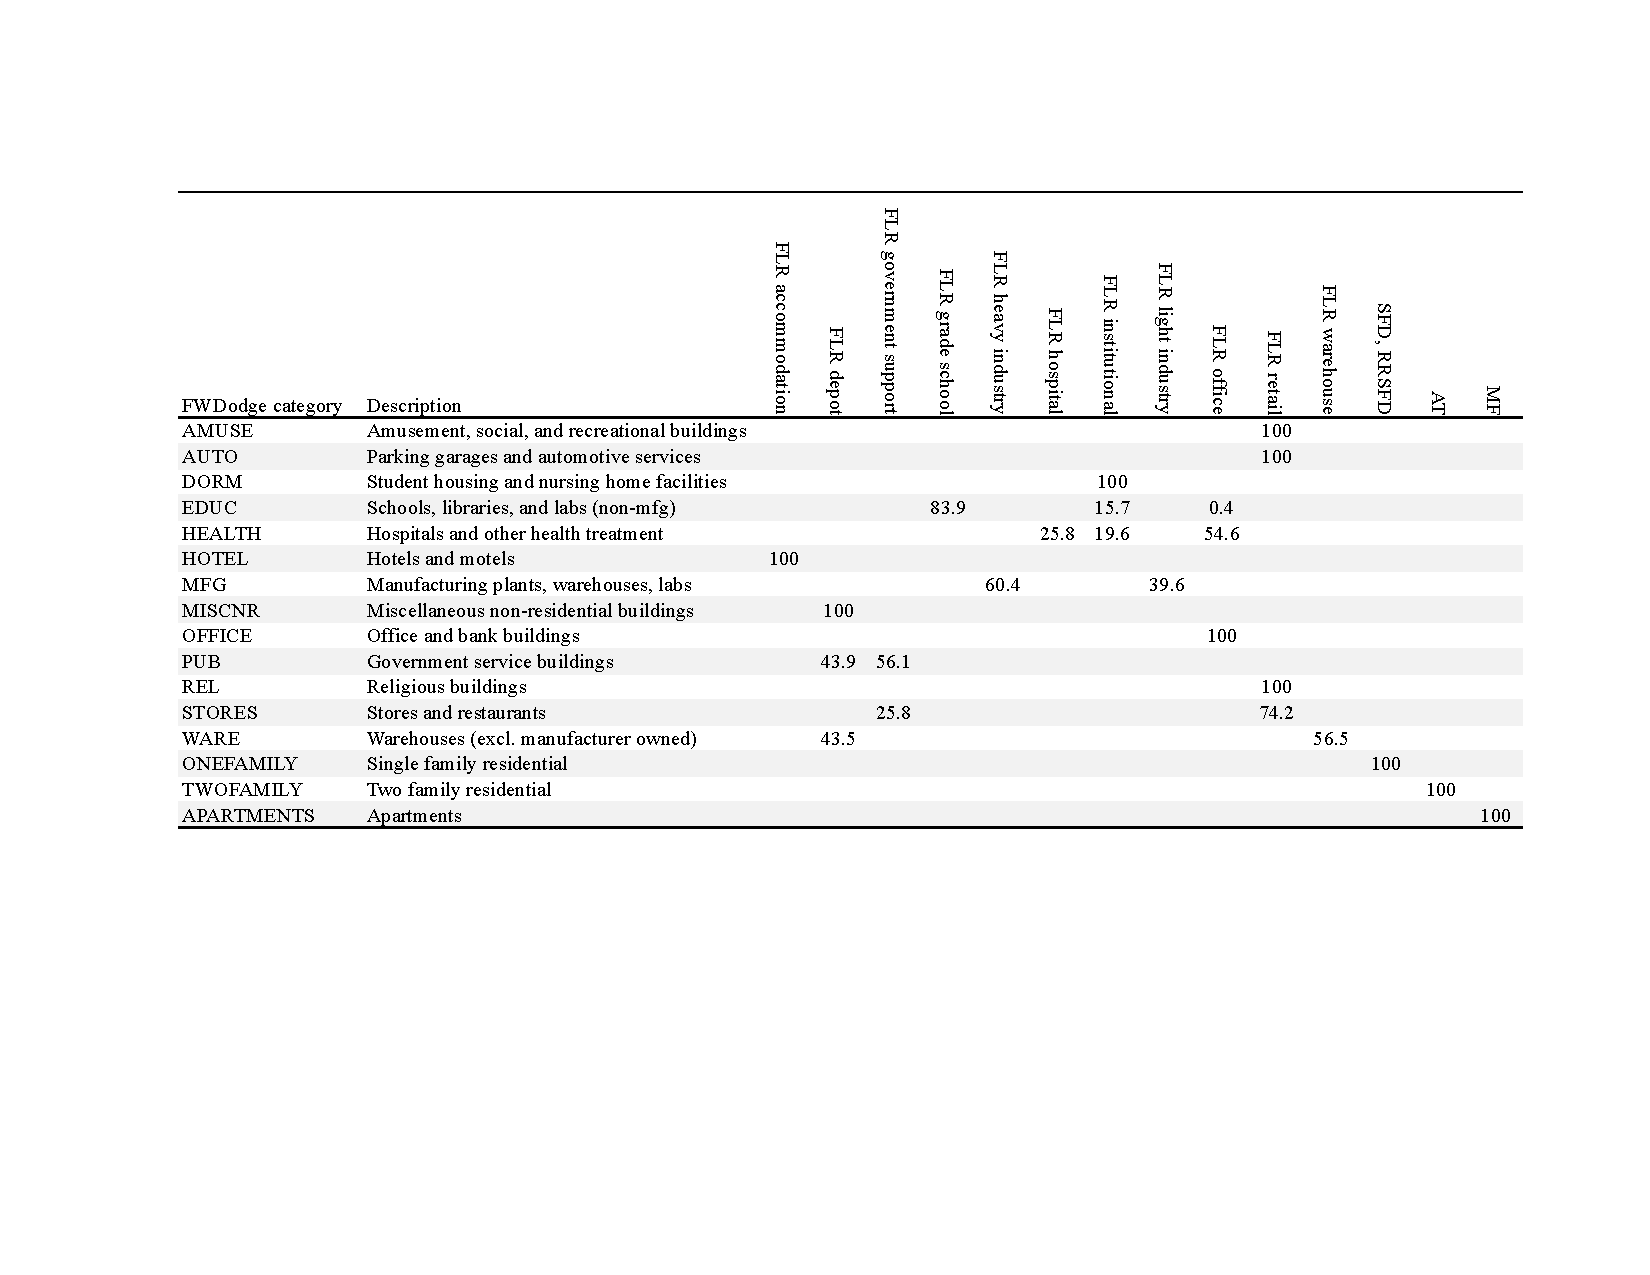
\includegraphics[scale=0.95, trim=28mm 70mm 20mm 32mm, clip]{ald/building-space-mapping} % trim=l b r t
\end{sidewaystable}

\begin{figure}
\centering
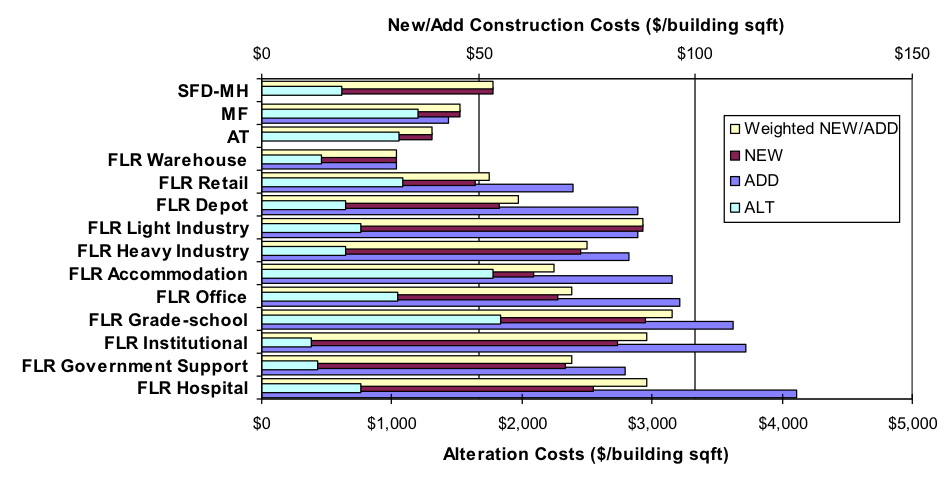
\includegraphics[scale=0.45]{ald/average-construction-costs}
\caption{Statewide average construction costs}\label{fig:average-construction-costs}
\end{figure}

\subsection{Modelwide Floorspace Value Decrease Factors (Df)}\label{sec:ald-floorspace-decrease-factors}   % 5.5.2
Residential and non-residential floorspace decrease factors were computed by comparing the average floorspace construction values produced by the ED module (prior to current NED model) for the period between 1990 and 2000, with the value of the change in floorspace computed from the FW Dodge data for the same period. The latter was calculated by multiplying the change in square footage computed from the FW Dodge data for each floorspace category by the unit construction cost rates estimated in Section \ref{sec:ald-unit-cost-rates}. The resulting decrease factors estimated in this way were 0.12 for residential and 0.39 for nonresidential.

Comparison of forecast and independent data in this way is rational but not a very rigorous exercise, but required in the face of limited data. In 2010, after early use of the model indicated that non-residential floorspace availability limitations from ALD were contributing to AA module convergence issues over time, these coefficients were revisited. As such, during calibration it was felt that a reduction in the non-residential factor was a reasonable action. Under this effort, the residential factor of 0.12 was applied to both residential and non-residential space types, significantly reducing the non-residential demolition. Some further sensitivity testing of this value may be of useful.

The values currently used by ALD are 0.12 for residential and nonresidential value. These Df values are stored in ALDResCoefficients.csv and ALDNresCoefficients.csv, respectively, which are found in the ``inputs/parameters'' folder.


\subsection{Land Capacity Calculation Parameters}\label{sec:ald-capacity-parameters}  % 5.5.3
The values of the Land Capacity Calculation parameters discussed in Section \ref{sec:ald-step2}, after S2 validation, including the dispersion parameter ($\lambda_p$), size term and coefficient ($size_f$, $stc$), are shown in Table \ref{tab:land-capacity-parameters}. In validation, significant adjustments were also made to the exogenous inputs of the compatibility matrix and FAR data. The $sizef$ term represents modelwide land area devoted to each floorspace type, developed from a modelwide GIS 30m grid coverage of built form (Development Type and Quantity of space) synthesized for the SWIM2 LD module.
% [10]

\begin{table}[!t]  % 5-3
\centering
\caption{ALD land capacity function parameters}\label{tab:land-capacity-parameters}
\begin{tabular}{llr}
\hline
Parameter & Description & Value \\
\hline
$\lambda_p$ & Dispersion parameter & 0.075 \\
stc & Size parameter & 1 \\
$size_f$ & FLR MH & 135,895,174 \\
 & FLR MF & 253,651,065 \\
 & FLR AT & 111,905,458 \\
 & FLR SFD & 1,385,141,602 \\
 & FLR RRMH & 82,164,425 \\
 & FLR RRSFD & 453,931,807 \\
 & FLR Accommodation & 29,262,691 \\
 & FLR Depot & 53,476,910 \\
 & FLR Government support & 111,166,124 \\
 & FLR Grade-school (K12) & 165,712,129 \\
 & FLR Heavy industry & 21,409,696 \\
 & FLR Hospital & 35,095,111 \\
 & FLR Institutional & 80,154,397 \\
 & FLR Light industry & 184,975,915 \\
 & FLR Office & 317,827,388 \\
 & FLR Retail & 193,736,194 \\
 & FLR Warehouse & 135,895,174 \\
\hline
\end{tabular}
\end{table}


\subsection{Model Parameters for Allocating Modelwide Construction Dollars into Regional Dollar Value Increases and Decreases}\label{sec:ald-increase-decrease}   % 5.5.4
ALD parameters were calibrated for functions that split ED (Now NED) module model wide residential and nonresidential construction dollars into region-level dollar increases and decreases (see \S\ref{sec:ald-step1}). For the purposes of S2 calibration, data from the Bureau of Economic Analysis' Regional Economic Information System (REIS) was used to measure activity. Employment was used as the measure of activity related to non-residential floorspace. Population was used as the measure of activity related to residential floorspace.

In S3 calibration, AA activity data will be used. The parameters for the increase and decrease functions were calibrated simultaneously using evolutionary algorithms. A population of 2000 parameter combinations was generated at random from a set of defined parameter bounds and run through 42 evolutionary steps to find the best fitting parameter combination. In each evolutionary step, increases and decreases were calculated and summed to calculate a net change by region.

The RMSE error between the calculated regional net changes and the regional changes calculated from the FW Dodge data was used as a fitness measure to identify the best fitting parameter combinations. The best fitting combinations were then modified through ``crossovers'' or ``mutations'' to produce a new population of 2000 parameter combinations used in the next step. Figure \ref{fig:residential-parameter-convergence} shows an example of convergence of residential floorspace increase function parameters. Figure \ref{fig:fwdodge-target-convergence} shows a corresponding example of the convergence of model net results to the FW Dodge target values for four regions. The resulting alternative specific constants are included in Tables \ref{tab:nonresidential-construction-asc} and \ref{tab:residential-construction-asc} for nonresidential and residential floorspace types, respectively (note that the Depot field was dropped for implementation with AA). The values for the four Cobb-Douglas production parameters are shown in Table \ref{tab:coff-douglas-parameters}.

\begin{sidewaystable}
\centering
\caption{Alternative-specific constants to allocate non-residential regional construction}\label{tab:nonresidential-construction-asc}
\small
\begin{tabular}{lrrrrrrrrrrr}
\hline
       & Accom- &       & Gov't   & Grade  & Heavy    &          & Institu- & Light    &        &        & Ware- \\
Region & modation   & Depot & Support & school & industry & Hospital & tional   & industry & Office & Retail & house \\
\hline
\multicolumn{12}{c}{Increase (inputs/parameters/ALDAsc1.RgFn.csv)} \\
\hline
Astoria\_LincolnCity & 0.944702 & 0.235614 & -0.259910 & 0.207471 & -2.907440 & 0.432939 & -0.081280 & -1.401530 & -0.741630 & 0 & -0.80103 \\
\gray BakerCity\_JohnDay & 0.586089 & 1.625532 & 1.801039 & 1.407736 & 1.504913 & 1.514356 & 1.926353 & 0.767333 & 0.735611 & 0 & -0.21093 \\
Bend & -0.884470 & 0.423798 & -0.349120 & 0.394332 & -1.880110 & -0.661790 & -1.066460 & -2.156670 & -0.397320 & 0 & -2.45611 \\
\gray Eugene & 0.699288 & 0.948542 & -1.294870 & -0.517360 & -1.251130 & 0.616967 & -0.096580 & -0.903660 & 0.458251 & 0 & -1.07190 \\
Eureka\_Brookings & 0.183214 & 0.072535 & 0.413877 & -0.792110 & -1.361930 & 0.714911 & 0.367652 & -0.367840 & -1.051680 & 0 & -0.81388 \\
\gray KlamathFalls\_Burns & 2.007493 & 0.904102 & 0.418304 & -0.045670 & -2.060080 & 1.614082 & 0.350857 & 0.120022 & 0.476692 & 0 & -0.56112 \\
Lewistown & 1.140614 & 1.039634 & 0.021470 & 1.676284 & -0.949050 & 1.471895 & 0.627516 & -1.017900 & 0.443534 & 0 & -0.66874 \\
\gray Longview\_Centralia & 0.145686 & 0.783508 & -0.723700 & -0.682170 & -0.822890 & 0.524477 & -1.092800 & -1.209510 & -0.484420 & 0 & -0.81174 \\
Medford\_GrantsPass & -0.008700 & -0.121280 & -0.623880 & -0.288720 & -0.944310 & 0.050372 & -0.001280 & -0.684090 & -0.257270 & 0 & -1.07863 \\
\gray Ontario\_Boise & 0.277807 & 0.494493 & -0.394450 & 0.146705 & -0.856080 & -0.350780 & -0.223810 & -0.876460 & 0.371850 & 0 & -1.44383 \\
Portland\_Vancouver & 0.086280 & 1.083125 & -1.308010 & -0.080430 & -0.828400 & -1.003140 & -0.586460 & -0.067400 & -0.086880 & 0 & -1.14624 \\
\gray Salem & 0.687471 & 1.323692 & -0.206050 & 0.244056 & -2.442220 & 0.217611 & -0.171280 & -2.377680 & -0.019380 & 0 & -0.99943 \\
TheDalles & -1.261090 & -0.51397 & -0.821790 & 0.332557 & -2.600690 & 1.032134 & 0.389188 & -3.854760 & -0.361730 & 0 & -1.24701 \\
\gray Yakima\_Pendleton & 0.483384 & 1.80530 & -0.398530 & 1.823500 & 0.272279 & 0.328345 & 1.068840 & 0.151031 & 0.850889 & 0 & -0.50899 \\
Yreka\_Redding & -0.096830 & -0.16398 & 0.622854 & 0.014584 & -1.37370 & 0.844414 & 1.112208 & -2.005020 & 0.295520 & 0 & -0.95297 \\
\hline
\multicolumn{12}{c}{Decrease (inputs/parameters/ALDAsc2.RgFn.csv)} \\
\hline
\gray Astoria\_LincolnCity & 2.763757 & -0.854408 & 0.550963 & -0.588357 & 2.171298 & -0.293591 & -0.729383 & 1.650154 & 0.827490 & 0 & -0.810913 \\
BakerCity\_JohnDay & -0.891268 & 1.010798 & 2.249196 & 2.157934 & 1.961006 & -1.042788 & 1.813892 & -0.465579 & 0.459310 & 0 & -1.913085 \\
\gray Bend & -0.460973 & 2.013159 & 2.660423 & 3.029211 & 2.405165 & 0.022755 & 0.053865 & 2.891694 & 1.527273 & 0 & -1.002809 \\
Eugene & -0.040206 & 2.570598 & -3.038275 & 0.235208 & 1.123078 & 2.402918 & -0.522408 & -0.052002 & 0.954050 & 0 & 0.541387 \\
\gray Eureka\_Brookings & 1.101352 & 0.885427 & 1.274713 & 0.741928 & 3.300662 & 0.772333 & 1.338762 & 3.018789 & 1.374824 & 0 & -0.496001 \\
KlamathFalls\_Burns & 0.781087 & 0.145467 & -0.085089 & -0.134997 & -0.002645 & 0.367056 & -1.208864 & 0.117831 & -0.319939 & 0 & -2.070174 \\
\gray Lewistown & 1.274683 & 1.499027 & 0.648288 & 2.126220 & 1.051077 & 0.914092 & -0.326581 & -0.350138 & 0.496095 & 0 & -0.821363 \\
Longview\_Centralia & 0.393504 & 1.158247 & -0.788388 & 0.676693 & 1.232855 & 1.975634 & -2.210476 & 1.070667 & 0.726616 & 0 & -0.175315 \\
\gray Medford\_GrantsPass & -0.147762 & 0.387470 & -0.288341 & 0.058904 & 2.180457 & -1.012891 & 1.545078 & 2.765504 & -0.164663 & 0 & 0.073767 \\
Ontario\_Boise & 0.584221 & 1.205850 & -0.251980 & -1.078799 & 2.275093 & 0.240065 & -0.487524 & 1.986376 & -0.335838 & 0 & 0.519281 \\
\gray Portland\_Vancouver & 1.363668 & 3.348070 & 0.122153 & 0.825876 & -0.962027 & -2.057667 & 0.743412 & 0.649737 & 1.054240 & 0 & 0.410136 \\
Salem & -0.082270 & 0.369023 & 1.562376 & 1.748439 & 0.128730 & 0.642501 & -0.449637 & -0.071461 & 0.692468 & 0 & -1.009280 \\
\gray TheDalles & -2.619944 & -2.514178 & -3.461466 & -3.148120 & -1.094045 & -3.291059 & -2.679318 & 3.974732 & -1.877617 & 0 & -2.478947 \\
Yakima\_Pendleton & -1.287373 & -1.349710 & -1.908386 & 2.254272 & 2.243717 & -1.789344 & 2.383304 & 2.847587 & 0.956473 & 0 & -1.576993 \\
\gray Yreka\_Redding & 1.226759 & -0.823016 & 1.439139 & 1.297564 & 0.675903 & 2.622162 & -0.211855 & 0.785988 & 1.974681 & 0 & 0.561401 \\
\hline
\end{tabular}
\end{sidewaystable}  % 5-4
\begin{table}
\centering
\caption{Alternative-specific constants to allocate residential regional construction}\label{tab:residential-construction-asc}
\begin{tabular}{lrrrrrr}
\hline
Region & MH & MF & AT & SFD & RRMH & RRSFD \\
\hline
\multicolumn{7}{c}{Increase (inputs/parameters/ALDAsc1.RgFr.csv)} \\
\hline
Astoria\_LincolnCity & 0.599185 & -0.09141 & 0.128806 & 0 & 0.32678 & 0.208994 \\
\gray BakerCity\_JohnDay & -0.28148 & -0.27616 & -0.43235 & 0 & -0.27724 & -0.34203 \\
Bend & 0.516327 & -0.53798 & -0.08595 & 0 & 0.838234 & 0.705884 \\
\gray Eugene & 0.117779 & 0.386703 & 0.844898 & 0 & -0.20865 & 0.002161 \\
Eureka\_Brookings & -0.06574 & -3.14471 & -3.61438 & 0 & -0.14144 & 0.498804 \\
\gray KlamathFalls\_Burns & 0.260061 & -0.22102 & 0.365183 & 0 & 0.421043 & 0.180597 \\
Lewistown & -0.21071 & -0.0555 & -0.01667 & 0 & -0.46303 & 0.319172 \\
\gray Longview\_Centralia & 0.271002 & -0.43668 & -0.34781 & 0 & 0.264514 & 1.194059 \\
Medford\_GrantsPass & 0.638162 & 0.274419 & 0.659648 & 0 & 0.395957 & 0.306998 \\
\gray Ontario\_Boise & -0.15147 & -0.94255 & -0.60234 & 0 & -1.02368 & 0.039501 \\
Portland\_Vancouver & 0.056183 & 0.073551 & 0.083727 & 0 & -0.73026 & 0.168127 \\
\gray Salem & 0.330187 & 0.338436 & 0.381144 & 0 & -0.20455 & 0.058002 \\
TheDalles & 0.448967 & -0.12737 & -0.0613 & 0 & 0.656301 & 1.422753 \\
\gray Yakima\_Pendleton & -0.36111 & -0.34582 & -0.45934 & 0 & -0.86607 & 0.432256 \\
Yreka\_Redding & -0.09976 & -0.24731 & -1.02394 & 0 & 0.283882 & 0.943806 \\
\hline
\multicolumn{7}{c}{Decrease (inputs/parameters/ALDAsc2.RgFr.csv)} \\
\hline
\gray Astoria\_LincolnCity & -1.84316 & -2.11438 & -3.64243 & 0 & -0.34124 & 0.111757 \\
BakerCity\_JohnDay & -2.84376 & -2.54353 & -3.50431 & 0 & -3.5544 & -2.39588 \\
\gray Bend & -2.31471 & -2.72093 & -2.86904 & 0 & -0.16878 & 1.979141 \\
Eugene & -2.09872 & -2.08561 & -1.92973 & 0 & -3.51411 & -0.59056 \\
\gray Eureka\_Brookings & -0.72992 & 0.928168 & 1.34931 & 0 & -3.59163 & 2.059602 \\
KlamathFalls\_Burns & -0.7994 & -2.39492 & -1.91467 & 0 & -2.25349 & -0.95675 \\
\gray Lewistown & -2.24869 & 0.179987 & -3.12329 & 0 & -1.48853 & -1.38146 \\
Longview\_Centralia & -2.3721 & -2.68488 & -1.009 & 0 & -1.44889 & 3.038585 \\
\gray Medford\_GrantsPass & -1.02841 & 0.355648 & -2.98606 & 0 & 0.255433 & 0.244647 \\
Ontario\_Boise & -0.05595 & -1.92675 & -0.26284 & 0 & -0.67294 & 3.677403 \\
\gray Portland\_Vancouver & -2.94502 & -3.14238 & -1.00111 & 0 & -3.17513 & 3.70538 \\
Salem & -3.3574 & -0.15295 & -0.62065 & 0 & -2.34857 & -2.15255 \\
\gray TheDalles & -1.2888 & -1.5701 & -2.09202 & 0 & -1.66081 & 1.975529 \\
Yakima\_Pendleton & -1.36691 & -0.85531 & -0.24308 & 0 & -1.40415 & 3.92212 \\
\gray Yreka\_Redding & -0.20314 & -1.31216 & -2.26709 & 0 & -2.96348 & 3.482707 \\
\hline
\end{tabular}
\end{table}   % 5-5

\begin{figure}[!t]
\centering
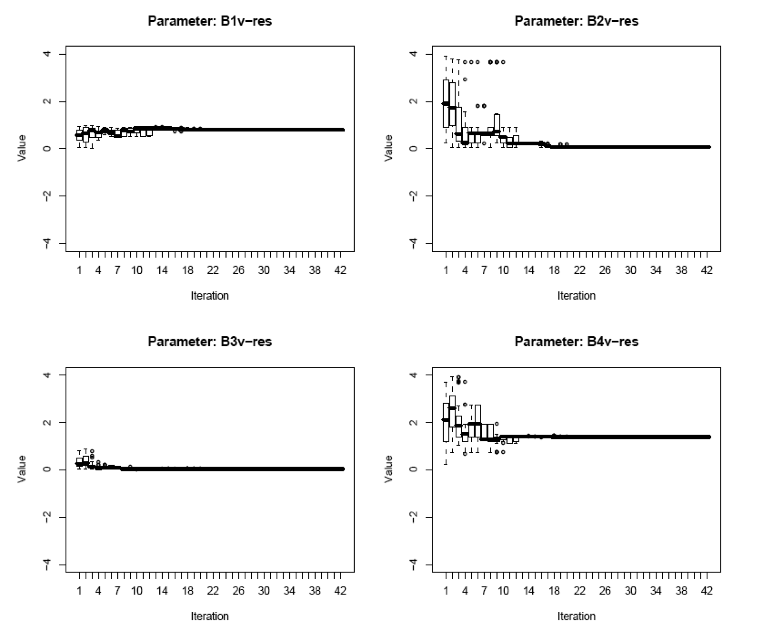
\includegraphics[width=6in]{ald/residential-parameter-convergence}
\caption{Convergence of residential parameter values}\label{fig:residential-parameter-convergence}
\end{figure}

\begin{figure}[!t]
\centering
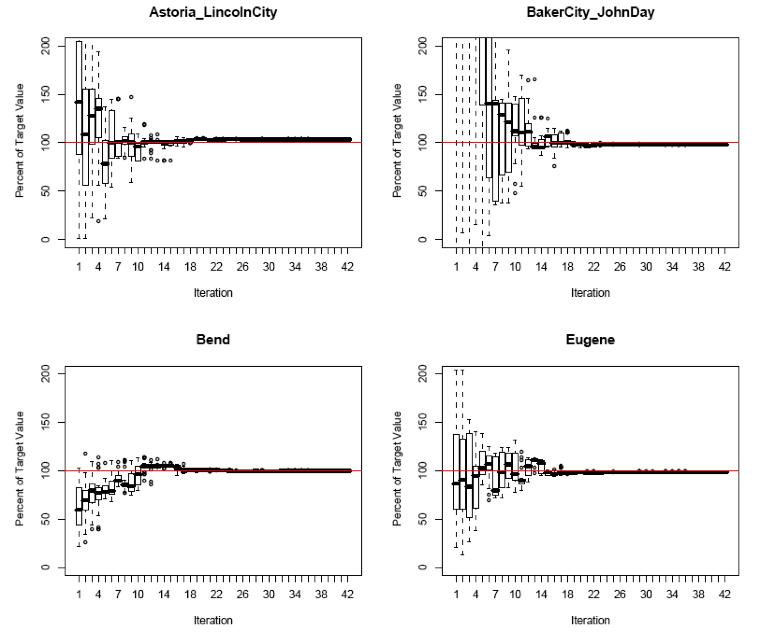
\includegraphics[width=6in]{ald/fwdodge-target-convergence}
\caption{Convergence of model results to FW Dodge target values}\label{fig:fwdodge-target-convergence}
\end{figure}

During 2015 S3 review of the modelwide construction dollars over time it was learned that ALD was far too sensitive to changes in regional activity from ALD. To counteract this, judgment from the team was applied. The parameters estimated above had an exponential term of approximated 2 (2.36 for non-residential and 1.96 for residential) on the activity change side of Equation \ref{eq:5.02}. After through review and testing it was determined that a more appropriate value for this term was a required a reduction by approximately one order of magnitude. Therefore, both residential and non-residential $\beta_{4v}$ parameters were set to 0.2 (this is reflected in Table \ref{tab:coff-douglas-parameters}).

\begin{table}   % 5.6
\centering
\caption{ALD Cobb-Douglas parameters}\label{tab:coff-douglas-parameters}
\begin{tabular}{clrr}
\hline
Parameter & Description & Nonresidential & Residential \\
\hline
$\beta_{1v}$ & Activity proportion additive term & 0.278924 & 0.707674 \\
$\beta_{2v}$ & Activity change proportion additive term & 1.968482 & 1.608066 \\
$\beta_{3v}$ & Activity proportion power & 0.399309 & 0.167152 \\
$\beta_{4v}$ & Activity change proportion power & 0.2 & 0.2 \\
\hline
\end{tabular}
\end{table}

Further, after this review it was determined that the decreasing set of parameters were likely incorrect as well. However, since there is far less data and information on how floorspace is converted (reduced and modified), the team opted to use the identical set of parameters used for the allocation of increase in dollars as in decrease. This was deemed acceptable, since this stage of the model is only working on total construction dollars by the 15 ALD regions; producing 30 highly aggregate values (15 for residential and 15 for non-residential) across the entire model area. The decision being that the level of precision at this level is not as great of a concern as it would be at more disaggregate decision points in the model.
  

\subsection{Model Parameters for Allocating Regional Dollar Increases and Decreases into Floorspace Types}\label{sec:ald-allocate-inc-dec}   % 5.5.5
The search space to find the best fit of parameters for the allocation of regional dollar development changes into floorspace type (see \S\ref{sec:ald-step2}) was very large, because of the significant number of alternative specific constants. Both the increase and decrease functions require an alternative specific constant for every combination of region and floorspace type. In order to get convergence and to ``maximize'' the share of ``behavior'' explained by the model parameters vs. the alternative specific constants, the process of calibrating this step was split into two parts. In the first part, the range of possible values for the alternative specific constants was constrained. 36 evolutionary steps were run to get the best fit results for the parameters. The best results from the first part were then processes through a second round of 25 evolutionary steps where the alternative specific constants were varied through a wider range of values. Figure \ref{fig:bend-floorspace-convergence} shows an example of the convergence of the proportional distribution of model net floorspace change to the FW Dodge target proportions for the Bend region. Tables \ref{tab:floorspace-allocation-parameters} and \ref{tab:floorspace-asc} show estimated parameter values.

\begin{figure}
\centering
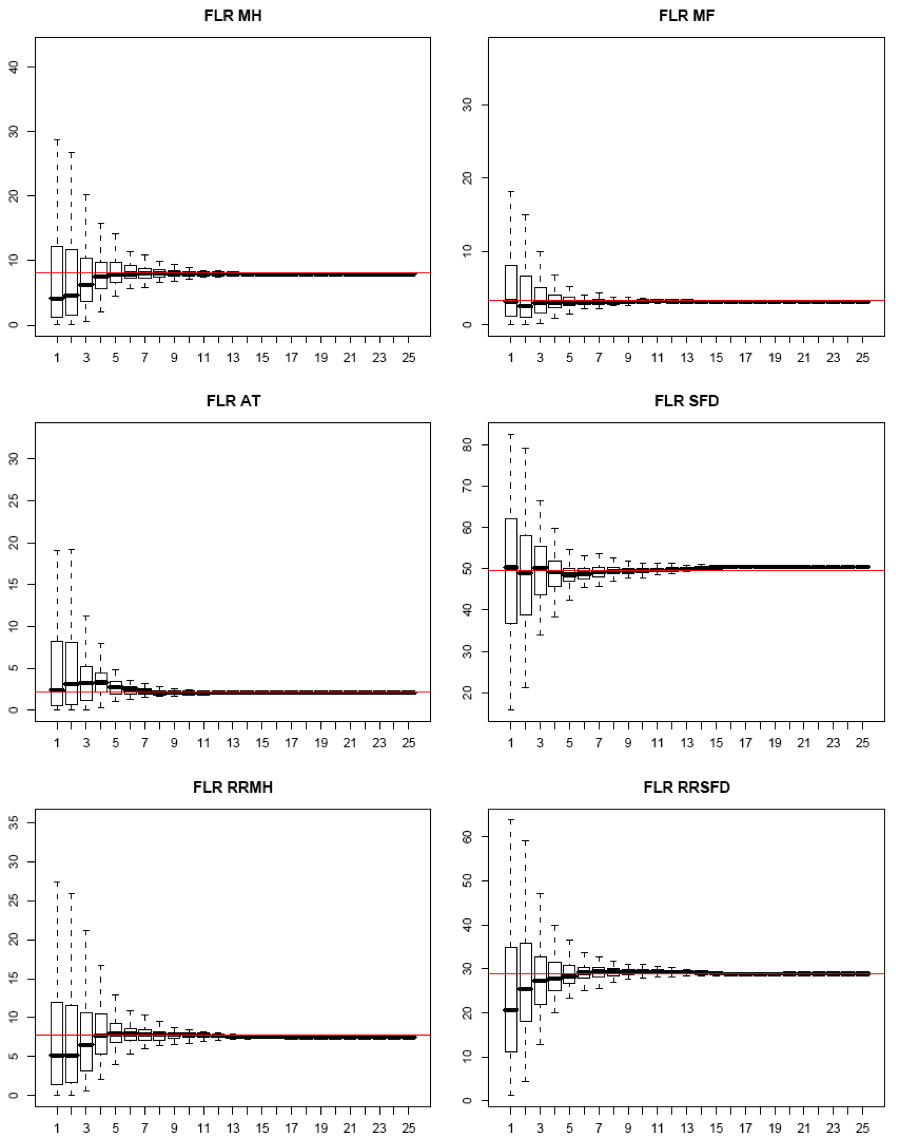
\includegraphics[width=6in]{ald/bend-floorspace-convergence}
\caption{Convergence of Bend Region model floorspace results to FWDodge target values}
\label{fig:bend-floorspace-convergence}
\end{figure}

\begin{table}[!t]    % 5-7
\centering
\caption{ALD parameters for allocation to floorspace types}\label{tab:floorspace-allocation-parameters}
\begin{tabular}{lclrr}
\hline
Category & Parameter & Description & Increase & Decrease \\
\hline
Nonresidential & $\lambda_{q1}, \lambda_{q2}$ & Dispersion parameter & 0.577946 & 0.309236 \\
 & $\beta_{q1}, \beta_{q3}$ & Sensitivity to vacancy rate: \\         
 & & FLR Accommodation & -0.448740 & -1.390874 \\
 & & FLR Depot (removed in AA) & -0.685066 & -1.770418 \\
 & & FLR Government Support & -0.717076 & -1.998696 \\
 & & FLR Grade-school & -1.081031 & -1.048652 \\
 & & FLR Heavy Industry & -2.992417 & -0.667520 \\
 & & FLR Hospital & -0.463261 & -1.030110 \\
 & & FLR Institutional & -0.387125 & -1.058415 \\
 & & FLR Light Industry & -2.197701 & -1.830717 \\
 & & FLR Office & -2.128987 & -2.648114 \\
 & & FLR Retail & -0.509895 & -1.394915 \\
 & & FLR Warehouse & -1.922216 & -1.823896 \\
 & $\beta_{q2}, \beta_{q4}$ & Sensitivity to prior year proportion & 0.874475 & 0.932353 \\
\hline
Residential & $\lambda_{q1}, \lambda_{q2}$ & Dispersion parameter & 1.016924 & 1.48071 \\
 & $\beta_{q1}, \beta_{q3}$ & Sensitivity to Vacancy rate: \\
 & & FLR MH & -2.68199 & 2.09219 \\
 & & FLR MF & -3.84517 & 2.71393 \\
 & & FLR AT & -3.60789 & 2.21573 \\
 & & FLR SFD & -2.24556 & 1.47095 \\
 & & FLR RRMH & -1.49781 & 1.55033 \\
 & & FLR RRSFD & -1.97620 & 3.11092 \\
 & $\beta_{q2}, \beta_{q4}$ & Sensitivity to prior year proportion & 0.993564 & 0.881172 \\
\hline
\end{tabular}
\end{table}

As with the previous section, S3 review conducted in 2015 showed that ALD region construction dollar increase and decreases did not match reasonable expectations. The issue was that any given ALD region could gain vastly more or substantially less construction activity over time than their size suggested. The calibrated parameters appeared to work for the calibrated base year, but then would become unstable over the course of the model. To adjust for this, model runs were made over the 30 year model horizon. Relative size targets for each ALD region were established over a history of census and employment information. The relative size by population over time of each ALD region was used as a guide or target residential construction dollars, and employment over time was used for non-residential construction dollars. An iterative process was then conducted where full SWIM model runs were done with successively iterating the parameter values found in Table \ref{tab:floorspace-asc}. This was conducted for several months until a final set of ALD region specific constants were established that held the regional construction dollar allocation in relative balance overtime. The model is still reactive to changes from scenarios, but is now better balanced to match high level expectations under the reference condition. The resulting parameters are shown in Table \ref{tab:floorspace-asc}.
 
\begin{table}
\centering
\caption{ALD allocation to floorspace types alternative specific constants}\label{tab:floorspace-asc}
\begin{tabular}{lcccc}
\hline
 & \multicolumn{2}{c}{Decrease} & \multicolumn{2}{c}{Increase} \\
Region & Residential & Non-residential & Residential & Non-residential \\
\hline
Astoria\_LincolnCity & 0.37 & 0.46 & 0.37 & 0.46 \\
\gray BakerCity\_JohnDay & 0.19 & 0.20 & 0.19 & 0.20 \\
Bend & 0.55 & 0.63 & 0.55 & 0.63 \\
\gray Eugene & 1.19 & 1.16 & 1.19 & 1.16 \\
Eureka\_Brookings & 0.55 & 0.60 & 0.55 & 0.60 \\
\gray KlamathFalls\_Burns & 0.21 & 0.25 & 0.21 & 0.25 \\
Lewistown & 0.48 & 0.67 & 0.48 & 0.67 \\
\gray Longview\_Centralia & 0.51 & 0.59 & 0.51 & 0.59 \\
Medford\_GrantsPass & 0.74 & 0.81 & 0.74 & 0.81 \\
\gray Ontario\_Boise & 1.58 & 1.92 & 1.58 & 1.92 \\
Portland\_Vancouver & 2.76 & 2.09 & 2.76 & 2.09 \\
\gray Salem & 1.49 & 1.43 & 1.49 & 1.43 \\
TheDalles & 0.21 & 0.28 & 0.21 & 0.28 \\
\gray Yakima\_Pendleton & 1.52 & 1.86 & 1.52 & 1.86 \\
Yreka\_Redding & 0.80 & 0.88 & 0.80 & 0.88 \\
\hline
\end{tabular}
\end{table}


\subsection{Model Parameters for Allocating Regional Floorspace Decreases and Increases to Alpha zones}\label{sec:ald-inc-dec-alpha}   % 5.5.6
The parameters influencing the zonal-level decrease and increase of floorspace by type, described in Sections \ref{sec:ald-step3} and \ref{sec:ald-step4}, were calibrated against the FW Dodge county change in net floorspace stock. In other words, upon completion of the net change in floorspace by alpha zone and type, the results are summed to the county level and compared with the FW Dodge data. As with the previous two steps, an evolutionary algorithm was used to calibrate the parameters. Unlike the other steps, however, there are no alternative specific constants, so the number of parameters to calibrate is smaller (but not small). This allowed there to be fewer evolutionary rounds. This was also necessary because these models have many more computations and require significantly more computing time per round. Only twelve evolutionary rounds were used. The results are not nearly as good as in the previous two steps. This is to be expected in part because this step creates a substantial disaggregation of the results. It is expected that this will improve in the S3 calibration. Resulting parameter values are shown in Table \ref{tab:zonal-floorspace-alloc}.

\begin{table}  % 5.9
\centering
\caption{ALD zonal floorspace allocation parameters}\label{tab:zonal-floorspace-alloc}
\begin{tabular}{lclrr}
\hline
Category & \multicolumn{2}{l}{Parameter} & Non-residential & Residential \\
\hline
Decrease & $\beta_{3f}$ & Prior year proportion dispersion & 1.963554 & 1.248889 \\
 & $\beta_{4f}$ & Price dispersion & -0.269004 & -0.271316 \\
\hline
Increase & $\beta_{5f}$ & Prior year proportion dispersion & 1.729279 & 1.160029 \\
 & $\beta_{6f}$ & Price dispersion & 0.347738 & 0.284712 \\
 & $\beta_{7f}$ & Prior year saturation factor & 0.248170 & 0.052244 \\
 & $\beta_{8f}$ & Prior year saturation dispersion & 5.817253 & 6.642847 \\
 & $\beta_{9f}$ & Prior year proportion additive term & 0.002111 & 0.000673 \\
\hline
\end{tabular}
\end{table}

\section{Inputs and Outputs}
ALD inputs and outputs are listed in Tables \ref{tab:ald-inputs} and \ref{tab:ald-outputs}. ALD requires current year construction activity values from NED and previous year activity (two-year) occupancy and price data from AA. Vacancy rates are calculated as the ratio of previous year AA occupied floorspace to previous year ALD total floorspace quantity. Zoning-based land capacities by alpha zone are exogenously developed for each year using GIS. Values for $ConsCostf$ are drawn from FWDodge construction starts data between 1990 and 2001 and were then inflated to 2009 dollars. Additional ALD definition files are also required to run the model. Detailed descriptions of several ALD input data are discussed in the remainder of this section.

ALD produces a current year floorspace inventory for AA (and for use in ALD in the next year). The agriculture and logging lands are adjusted in the AA file, as discussed in \S\ref{sec:ald-completing-inventory}. In addition to the outputs used by other modules, ALD prints a series of diagnostic files listed also in Table \ref{tab:ald-outputs}.

\begin{table}[!t]    % Table 5-10
\centering
\caption{ALD inputs}\label{tab:ald-inputs}
\begin{tabular}{p{4.8in}l}
\hline
Data element & Source \\
\hline
Modelwide construction activity \$ for residential (\$res) and nonresidential (\$nres) categories [construction\_forecast.csv] & NED \\
\gray Beta Zone activity demand (HHs and industry \$ by type) [ExchangeResults.csv] & Current year AA \\
Modelwide occupied floorspace (sqft) by floorspace category [ExchangeResults.csv] & Current year AA \\
\gray Unit prices for residential and nonresidential space in alpha zones [ExchangeResults.csv] & Current year AA \\
Building square footage by alpha zone (row) and floorspace type (col) [FloorspaceInventory.csv] & Previous year ALD \\
\gray Alpha-beta zone conversion [alpha2beta.csv] & SI \\
Modelwide space construction costs per square foot by floorspace type [ConstructionCosts.csv] & Exogenous \\
\gray Matrix of land square feet by alpha zone and zoning category (zonal input) [LandSQFTxzoning.csv] & SI \\
Matrix of floor to area ratios by floorspace type (rows) and zoning category (cols) [far.csv] & Exogenous \\
\gray Matrix of compatibility values (NP-0 to VH-1=best) by floorspace type (row) and zoning category (col) [zoning\_compatibility.csv] & Exogenous \\
Definition files [floorspace\_definitions][zoning\_definitions] & Exogenous \\
\gray Land Capacity Size term values [LandSQFTxFLR.csv] & Exogenous \\
\hline
\end{tabular}
\end{table}

% Table 5 11 ALD Outputs
\begin{table}[!t]    % Table 5-11
\centering
\caption{ALD outputs}\label{tab:ald-outputs}
\begin{tabular}{p{4.8in}l}
\hline
Description & Users \\
\hline
Building square footage (landsqft for agriculture and logging) by alpha zone (row) and floorspace type (col) [FloorspaceInventory.csv] & PT, next year ALD \\ 
\gray AA-format building square footage (landsqft for agriculture and logging) by alpha zone (row) and floorspace type (col) [FloorspaceI.csv] & AA \\
Floorspace type split within each zoning category [FloorspaceProportionsByZoning.csv] & Diagnostics \\
\gray Building space increase for each floorspace type in each alpha zone [Increments.csv][Increments\_Matrix.csv] & AA, diagnostics \\
Land sqft of each floorspace type in each alpha zone [LandAllocations.csv] & Diagnostics \\
\gray Building sqft zoning capacity of each floorspace type in each alpha zone [ResidentialCapacity.csv] [NonresidentialCapacity.csv] & Diagnostics \\
Ratio of floorspace after decrease (but before increase) to total floorspace capacity [CapacityUtilization.csv] & Diagnostics \\
\gray Building Msqft decrease of each floorspace type in each alpha zone [ResidentialDecrease.csv] [NonresidentialDecrease.csv] & Diagnostics \\
Decrease utility for each floorspace type in each alpha zone [ResidentialDecreaseUtilities.csv] [NonresidentialDecreaseUtilities.csv] & Diagnostics \\
\gray Building Msqft increase of each floorspace type in each alpha zone [ResidentialIncrease.csv] [NonresidentialIncrease.csv] & Diagnostics \\
Increase utility for each floorspace type in each alpha zone [ResIncreaseUtilities.csv] [NonresIncreaseUtilities.csv] & Diagnostics \\
\gray Building Msqft after decrease (before increase) of each floorspace type in each alpha zone  [ResQuantititesAfterDecrease.csv] [NonresQuantititesAfterDecrease.csv] & Diagnostics \\
Log file for ALD run [ald.Rout] & Diagnostics \\
\gray R workspace from most recent run [.RData] & Diagnostics \\
Matrix of alpha zone/floorspace types where capacity less than floorspace quantity (after decrease) [ResLowCapacity.csv] [NonresLowCapacity.csv] & Diagnostics \\
\hline
\end{tabular}
\end{table}

\subsection{Base year Floorspace Estimates}\label{sec:ald-baseyear-floorspace}  % 5.6.1
Floorspace is difficult to gather statewide at any sub-county level. To be consistent with the space needed for AA activities (see \S\ref{sec:aa-pc-allocation} on page \pageref{sec:aa-pc-allocation}), a modelwide floorspace inventory (by alpha zone) was synthesized for the base year to cover four categories:
\begin{itemize}
\item Residential building floorspace (building sqft).
\item Non-residential housing floorspace (building sqft).
\item Productive agricultural lands (land sqft).
\item Productive logging timberlands (land sqft). 
\end{itemize}

For residential building space, a use rate was applied to the alpha zone number of ACS 2005-2009 census (December 2010 summary file block group data release) dwelling units, both vacant and occupied. Rural residential types were distinguished based on percentage of units over one-acre lot size from ACS PUMA 2005-2009 dataset (ACR field) at the PUMA level. In urban areas, a separate urban and rural residential factor (census designation of urban and rural) was applied with an upper limit of 90 percent of the zone assigned to rural residential. The rates of sqft per household based on a regression analysis of the 2001 American Housing Survey (microdata) were applied to the resulting number of housing units by residential type.

% Table 5 12 Residential Space usage rates by dwelling type

For non-residential building space, an initial synthesized base year floorspace inventory was developed from the AA module space use rates (Table \ref{tab:employee-floorspace-use}) and zonal activity targets directly, as follows:
\begin{equation}  % 5.24
SQFT_{z,f} = UseRate_{a,f,LUI} \times ActivityTarget_{z,a}
\end{equation}
\noindent where:
\begin{align*}
SQFT_{f,z} &= \text{synthesized floorspace quantity (sqft) of floorspace type $f$ in zone $z$} \\
UseRate_{a,f,LUI} &= \text{target use of floorspace $f$ by activity $a$ in land use intensity category $LUI$} \\
 &~~~~~\text{for the zone (\S\ref{sec:ald-zoning-data})} \\
ActivityTarget_{z,a} &= \text{target quantity of activity $a$ in zone $z$ (2009 Census HHs and IMPLAN-based} \\
 &~~~~~\text{employment, see AA zonal activity targets in \S\ref{sec:aa-zonal-activity-targets})}
\end{align*} 

\begin{small}
\begin{longtable}{llrrrr}
\caption{\normalsize{Employee floorspace use rates by land use intensity (LUI) level}}\\
\hline
Activity\_short\_name & Floorspace & High & Medium & Low & VeryLow \\ \hline
\endfirsthead
\hline
Activity\_short\_name & Floorspace & High & Medium & Low & VeryLow \\ \hline
\endhead
\hline \multicolumn{6}{r}{\emph{Continued on next page}}
\endfoot
\hline
\endlastfoot\label{tab:employee-floorspace-use}
RES\_agmin\_ag* & FLR Agriculture & & 392,040 & 392,040 & 392,040 \\
RES\_forst\_log & FLR Logging & & 2,178,000 & 2,178,000 & 2,178,000 \\
RES\_offc\_off & FLR Office & 214 & 268 & 326 & 376 \\
ENGY\_elec\_hi & FLR Heavy Industry & 1178 & 690 & 703 & 953 \\
ENGY\_ngas\_hi & FLR Heavy Industry & 1178 & 690 & 703 & 953 \\
ENGY\_ptrl\_hi & FLR Heavy Industry & 1178 & 690 & 703 & 953 \\
ENGY\_offc\_off & FLR Office & 171 & 208 & 263 & 235 \\
CNST\_offc\_off & FLR Office & 187 & 224 & 260 & 262 \\
MFG\_food\_hi & FLR Heavy Industry & 412 & 351 & 661 & 725 \\
MFG\_htec\_hi & FLR Heavy Industry & & 508 & 750 & 621 \\
MFG\_hvtw\_hi & FLR Heavy Industry & 412 & 351 & 661 & 725 \\
MFG\_lvtw\_hi & FLR Heavy Industry & 412 & 351 & 661 & 725 \\
MFG\_wdppr\_hi & FLR Heavy Industry & & 482.5 & 785.5 & 870.5 \\
MFG\_food\_li & FLR Light Industry & & 776 & 1175 & 868 \\
MFG\_htec\_li & FLR Light Industry & & 508 & 750 & 621 \\
MFG\_hvtw\_li & FLR Light Industry & & 508 & 750 & 621 \\
MFG\_offc\_off & FLR Office & 187 & 224 & 260 & 262 \\
WHSL\_whsl\_ware & FLR Warehouse & 1719 & 1341 & 1340 & 984 \\
WHSL\_offc\_off & FLR Office & 163 & 212 & 221 & 250 \\
RET\_auto\_ret & FLR Retail & 554 & 570 & 580 & 565 \\
RET\_stor\_ret & FLR Retail & 443 & 456 & 464 & 452 \\
RET\_stor\_off & FLR Office & 126 & 164 & 180 & 117 \\
RET\_nstor\_off & FLR Office & 126 & 164 & 180 & 117 \\
TRNS\_trns\_ware & FLR Warehouse & 1720 & 1581 & 1929 & 1292 \\
TRNS\_trns\_off & FLR Office & 208 & 244 & 277 & 316 \\
INFO\_info\_off\_li & FLR Office & 259 & 278 & 293 & 221 \\
INFO\_info\_off\_li & FLR Light Industry & 259 & 278 & 293 & 221 \\
INFO\_info\_off & FLR Office & 259 & 278 & 293 & 221 \\
UTL\_othr\_off\_li & FLR Office & 171 & 208 & 263 & 235 \\
UTL\_othr\_off\_li & FLR Light Industry & 1178 & 690 & 703 & 953 \\
UTL\_othr\_off & FLR Office & 171 & 208 & 263 & 235 \\
FIRE\_fnin\_off & FLR Office & 146 & 169 & 212 & 242 \\
FIRE\_real\_off & FLR Office & 146 & 169 & 212 & 242 \\
HLTH\_hosp\_hosp & FLR Hospital & 248 & 278 & 250 & 230 \\
HLTH\_care\_inst & FLR Institutional & 252 & 257 & 242 & 238 \\
HLTH\_othr\_off\_li & FLR Office & 259 & 278 & 293 & 221 \\
HLTH\_othr\_off\_li & FLR Light Industry & 252 & 257 & 242 & 238 \\
K12\_k12\_k12 & FLR Grade-school & 732 & 744 & 872 & 733 \\
K12\_k12\_off & FLR Office & 149 & 174 & 194 & 214 \\
HiED\_hied\_off\_inst & FLR Office & 149 & 174 & 194 & 214 \\
HiED\_hied\_off\_inst & FLR Institutional & 197 & 240 & 253 & 247 \\
ENT\_ent\_ret & FLR Retail & 259 & 278 & 293 & 221 \\
HOSP\_acc\_acc & FLR Accommodations & 808 & 908 & 879 & 576 \\
HOSP\_eat\_ret\_acc & FLR Retail & 259 & 278 & 293 & 221 \\
HOSP\_eat\_ret\_acc & FLR Accommodations & 259 & 278 & 293 & 221 \\
SERV\_tech\_off & FLR Office & 259 & 278 & 293 & 221 \\
SERV\_site\_li & FLR Light Industry & 54 & 54 & 54 & 54 \\
SERV\_bus\_off & FLR Office & 259 & 278 & 293 & 221 \\
SERV\_nonp\_off\_inst & FLR Office & 259 & 278 & 293 & 221 \\
SERV\_nonp\_off\_inst & FLR Institutional & 259 & 278 & 293 & 221 \\
SERV\_stor\_ret & FLR Retail & 259 & 278 & 293 & 221 \\
GOV\_admn\_gov & FLR Government Support & 214 & 255 & 243 & 231 \\
GOV\_offc\_off & FLR Office & 192 & 220 & 232 & 222 \\
FGOV\_acct\_gov & FLR Government Support & 214 & 255 & 243 & 231 \\
SLGOV\_acct\_gov & FLR Government Support & 214 & 255 & 243 & 231 \\
CAP\_acct\_gov & FLR Government Support & 214 & 255 & 243 & 231 \\
CNST\_main\_xxx & N/A & 0 & 0 & 0 & 0 \\
CNST\_nres\_xxx & N/A & 0 & 0 & 0 & 0 \\
CNST\_othr\_xxx & N/A & 0 & 0 & 0 & 0 \\
CNST\_res\_xxx &  N/A & 0 & 0 & 0 & 0 \\ 
\end{longtable}
\end{small}
   % Table 5 13

Space use rates were not only based on activity, they were based on activity, job type and land use intensity by zone.  For employment, the activity targets used in the development of space are slightly more disaggregate than those used when running the model. For instance employees in the food service industry HOSP\_eat\_ret\_acc were assigned to either accommodation space or retail space depending on the presence of hotels in the zone (one hotel-restaurant employee for every two accommodation employees in the zone, unless there were not enough restaurant employees in the zone to satisfy this ratio). 

Activity targets used in the development of agriculture space and logging space are slightly different from the employment used to run the model. To estimate these types of space an inventory of land used for agriculture and logging was taken in account to identify the minimum acreage per employee of these resource-based production industries. The source of this information is explained below in the next few paragraphs of this section.  

Agricultural and logging lands are now inventoried in square feet, but were originally developed and inventoried in units of land area (acres). Acres of agriculture lands were identified from the 1997 Census of Agriculture for each county in the study area. Agriculture lands include acres of farmland defined in the 1997 census as cropland or other land (i.e., land in house lots, ponds, roads, wasteland), excluding woodlands and pasture-only non-croplands. Data omissions were estimated from other categories and/or prior 1992/1987 census data. Mining lands (quarries, strip mines, gravel pits), taken directly from 1990 USGS NLDC GIS land coverage, were added to the Agriculture lands.
%% [10]

County timberland\footnote{Timberland is defined by the USFS as Forest land capable of growing 20 cubic feet or more per acre per year (mean annual increment at culmination in fully stocked, natural stands) of industrial wood, and not in a reserved status through removal of the area from timber utilization by statute ordinance or administrative order; and not in a withdrawn status where it is pending consideration for reserved status.} acres were identified from the respective natural resource departments in each state (all data from the mid-1990's) to represent the long-term supply of harvestable forestland. These sources are listed in Table \ref{tab:timberland-data-sources}.

\begin{table}[!b]
\centering
\setlength\belowcaptionskip{3pt}
\caption{Sources of timberland data}\label{tab:timberland-data-sources}
\small
\begin{tabular}{p{6.2in}}
\hline
Timber Resource Statistics for Western Oregon 1999, US Department of Agriculture, Forest Service, Pacific Northwest Research Station, Resource Bulletin PNW-237 (Oct 2002); Table 3-Estimated area of timberland, by county and owner class, western Oregon (Jan 1997) \\
\gray Timber Resource Statistics for Eastern Oregon 1999, US Department of Agriculture, Forest Service, Pacific Northwest Research Station, Resource Bulletin PNW-238 (Dec 2002); Table 3-Estimated area of timberland, by county and owner class, eastern Oregon (1999) \\
Timber Resource Statistics for Eastern Washington, US Department of Agriculture, Forest Service, Pacific Northwest Research Station, Resource Bulletin PNW-RB-201 (revised Feb 1995); Table 3-Area of timberland outside National Forests, by county and owner, Eastern Washington (Jan 1992) \\
\gray Timber Resource Statistics for Western Washington, US Department of Agriculture, Forest Service, Pacific Northwest Research Station, Resource Bulletin PNW-RB-218 (1997); Table 10-Area of Timberland by county/owner (1992) \\
California Department of Forestry (CDF), California Forest and Rangeland Resources Assessment, Updated California Forest Statistic Abstract; Table G-27-Area of Timberland by county/owner (1994-1998) \\
\gray US Department of Agriculture, Forest Service, Forest Inventory and Analysis Database (FIADB); Table 2-Area of timberland by county and ownership class, for Idaho (1991) and Nevada (1989) \\
\hline
\end{tabular}
\end{table}


The allocation of these county estimates to alpha zones, used the distribution of agriculture, mining, range and forest lands (outside of urban areas), as identified in a mid-1990s 30m grid GIS land cover database of the study area. This land cover database was built primarily from the following sources. Additional details can be found in \cite{weidner04}:   % Ref 10 in v30

\begin{itemize}
\item Mid-1990s Pacific Northwest Ecosystem Research Consortium (PNWERC) data covering the Willamette Valley.
\item 1990 US Geological Survey (USGS) National Land Cover Dataset (NLCD).
\item 1995 DLCD Urban Growth Boundaries.
\item 1993 Portland Metro Regional Land Information System (RLIS).
\item 1993 Clark County Planning Department general land use coverage.
\item 1991 Western Oregon Industrial Forestland Ownership GIS coverage, Oregon State Department of Forestry.
\item Various 2002 Environmental Systems Research Institute (ESRI) GIS shape files (e.g., federal lands, landmarks, airports, schools, hospitals, water, census urban places).
\end{itemize}

Agriculture and logging lands were further constrained in the urban areas (those areas with over 10 percent land acres within the UGB). Resource-based production (non-office) employees in these two industries were only allowed to occur on land zoned as `rfor', `rnatrs' or `xagfor' (legacy zoning codes from previous iterations of ALD). Agriculture production employees were constrained to total acres of `rnatrs' plus `xagfor' in the zone, while the Logging production employees could use any of the three zoning coverages. These restrictions were set up inside of the employment synthesizer (see \S\ref{sec:aa-zonal-activity-targets} on page \pageref{sec:aa-zonal-activity-targets}), assuming nine acres for agriculture workers and 50 acres per forestry worker estimated from mid-1990s land inventory and employment data, as noted above. 

Once the employment was estimated for agriculture and logging by alpha zone, the space use rate shown in (Table \ref{tab:employee-floorspace-use}) was applied to obtain the initial floorspace estimate. A couple of quality control measures were applied to ensure that the floorspace estimation met the restrictions defined by the `xagfor' zoning. The details of the equations used to build the initial floorspace for all sectors are described in \citep{hbaspecto12}. 

% 5.6.2
\subsection{Zoning Data}\label{sec:ald-zoning-data}
In ALD, several zoning inputs are required. This includes a set of zoning categories, associated allowable floorspace types and maximum intensities (floor-area-ratios, FARs) and the amount of land (sqft) of each of these categories within each study area alpha zone. In the future, the user should be able to modify at least the GIS zoning coverage in future years. The 55 zoning categories, previously defined in Table \ref{tab:ald_zoning_cat}, match statewide generalized zoning codes from the Department of Land Conservation and Development (DLCD). 

The zoning code indicates the type and intensity of development allowed. Compatibility measures, on a scale of 0 to 1 (best), the likelihood of each floorspace type to occur within each zoning category. Maximum Floor-Area-Ratios are used to calculate the floorspace capacity allowed by the zoning coverage. Both were developed from expert judgment. Both inputs are very large and are not easily viewed in a document like this.  These conversion files can be found at reviewed in ``inputs/t0'', ``zoning/compatibility.csv'' and ``far.csv''.

The amount of land (sqft) of each zoning category within each study area alpha zone was originally developed from a GIS 30m grid coverage of previous zoning categories across the study area. This GIS coverage was then tabulated to result in the land area within each zoning category and alpha zone. In 2013, when the generalized zoning layers for the majority of the state became available, they were used to update all zones where coverage existed.  The data from the previous process was used for the handful of areas inside of Oregon that did not have the generalized coverage and for the model Halo region.

For the original base year four key zoning data sources were used to develop the GIS zoning coverage: 
\begin{itemize}
\item 1999 PNWERC for the Willamette Valley (Salem, Albany, Corvallis, Eugene).
\item Late 1980s DLCD for rural areas in Oregon.
\item 1995 Clark County (WA) and 1993 Portland Metro zoning data.
\item ESRI federal lands and reservation GIS coverage.
\item Land cover data on existing protected areas, water features and major transportation rights of way.
\end{itemize}

Initially, a zoning coverage was developed for the full study area, using LCDC in rural Oregon, ESRI protected Federal lands in rural halo and uany or ubigany in urban areas. Forest areas in the halo not directly protected were zoned rural residential (rres). Urban areas were bound by urban growth boundaries in Oregon, urban growth area in Clark County, WA and Census Designated Places elsewhere.

This initial coverage was updated with more detailed urban zoning data obtained from local MPOs and the PNWERC dataset. This urban layer added detailed local zoning data in the four Portland-Vancouver metropolitan area counties: Multnomah, Washington, Clackamas and Clark County, WA. Less detailed PNWERC zoning and density information was used to provide various zoning categories within the larger cities in the Willamette Valley including: Salem, Albany, Corvallis and Eugene. As a result of this layer, zoning in the larger urban areas was improved, while rural communities/centers and smaller Oregon and halo urban areas continue to assume a permissive zoning. Additionally, because of the mismatch between data sets, some areas along the edges of the larger cities are also zoned permissively.

Major water and transportation rights-of-way from a land cover GIS data were overlaid to bar development in these locations. An adjustment was also made in the Portland Metro area to correct the zoning of protected publicly owned lands (e.g., parks, schools, cemeteries). Any publicly owned lands within the Metro area (using RLIS parcel data) that had an agriculture/forest-type GIS land coverage were rezoned as urban public (originally zoned residential). Details on GIS processing to develop the zoning and land cover datasets can be found in \cite{weidner04}. Most of this information and process was then overwritten in 2013 when the generalized zoning layer from DLCD became available.

% 5.6.3
\subsection{Floorspace Quantity Calibration Targets}
FW Dodge purchased 1990-2000 building stock data was purchased for the 75-county study area (Oregon and Halo). Initially developed as a base year nonresidential floorspace estimate, but when inconsistencies were found with census activity, the FWDodge-based floorspace inventory's change in floorspace was used as a calibration target at a county level. The 12 FWDodge nonresidential building stock categories, including both vacant and occupied space, were disaggregated to the SWIM floorspace types (Table \ref{tab:floorspace-categories} on page \pageref{tab:floorspace-categories}) and to alpha zones, using 1998 employment estimates by industry and alpha zone (originally developed for the PI module). The primary FWDodge space categories that were split using employment estimates were:
\begin{itemize}
\item Split of institutional and office space from FWDodge education and health space types
\item Split of light and heavy industry from FWDodge industry space types
\item Government services use of FWDodge retail space
\item Split of depot space from FWDodge public and warehouse building stock
\item Split of FWDodge DORM space among residents (90 percent of space) and employees (10 percent)\footnote{FWDodge's DORM space accounts for roughly 0.5 percent of total residential and one percent of total nonresidential building stock in the study area in 1998. The chosen approach will assume ten percent of the FWDodge dorm building stock, which includes educational residence halls and nursing homes, are institutional space used by employees. The remaining 90 percent is assumed to be (multi-family) residential space. All prisons are included in governmental support employee space, while prisoners are housed in multi-family housing. Alternate approaches considered for dealing with group quarters ranged in complexity. Simplistically, the model could be structured to ignore the residential demands of all group quarters and simply allocate employees to utilize the entire space. A second more involved method would add a new floorspace category, DORM and a new HA household category, GroupQuarters. The floorspace would then be split among these uses, but allow more behavioral treatment than the institutional/multi-family space of the current approach.}
\end{itemize}

Initially an artificial floorspace estimate based on employment was generated by applying floorspace consumption rates, which varied by industry and land use intensity (originally developed for the PI module). The space rates (sqft per employee), shown in Table \ref{tab:floorspace-consumption-rates}, are based on Portland Metro data and engineering judgment with calibrating adjustments to match available FWDodge space (note that in SWIM2, Construction and home-based services industries do not consume floorspace). In this calibration process, government employment space consumption rates (including government use of retail space) were found to be roughly equivalent to office workers (200 sqft/employee). This is lower than expected, possibly due to 24 hour/day, seven day/week staffing of police and fire facilities, as well as a high level of mobile government workers that do not use much space. This would be expected to be offset somewhat by large public spaces (courthouses, city buildings, etc.). Land use intensity is calculated as a logged scale of combined 1998 population and employment per zone area (originally developed for the PI module). 

It should be noted that ALD calibration was done using floorspace targets developed for the PI module, which has since been replaced with the AA module. New floorspace targets and further calibration may be desired.

% Table 5 14 Floorspace Consumption Rates (sqft per employee)
\begin{sidewaystable}
\centering
\caption{Floorspace consumption rates (sqft per employee)}
\label{tab:floorspace-consumption-rates}
\small
\begin{tabular}{llrrrrr}
\hline
 & & \multicolumn{5}{c}{Land use intensity (LUI)} \\
\cline{3-7}
AA industry & Floorspace type & VeryHigh & ~~~High & Medium & ~~~~Low & Default \\
\hline
Accommodations & FLR accommodation & 690 & 770 & 850 & 800 & 800 \\
\gray Agriculture and mining--office & FLR office & 210 & 240 & 270 & 250 & 251 \\
Communication and utilities--light industry & FLR light industry & 600 & 660 & 750 & 710 & 705 \\
\rowcolor{gray!10}Communication and utilities--office & FLR office & 160 & 180 & 200 & 190 & 186 \\
Electronics and instruments--light industry & FLR light industry & 560 & 620 & 750 & 750 & 747 \\
\rowcolor{gray!10}Electronics and instruments--office & FLR office & 170 & 190 & 200 & 200 & 195 \\
FIRE business and professional services & FLR office & 140 & 150 & 170 & 160 & 161 \\
\rowcolor{gray!10}Food products--heavy industry & FLR heavy industry & 340 & 380 & 800 & 800 & 798 \\
Food products--light industry & FLR light industry & 560 & 620 & 1040 & 1040 & 1037 \\
\rowcolor{gray!10}Food products--office & FLR office & 170 & 190 & 200 & 200 & 195 \\
Government administration--government support & FLR government support & 170 & 190 & 210 & 200 & 200 \\
\rowcolor{gray!10}Government administration--office & FLR office & 170 & 190 & 200 & 200 & 195 \\
Health services--hospital & FLR hospital & 250 & 250 & 250 & 250 & 250 \\
\rowcolor{gray!10}Health services--institutional & FLR institutional & 200 & 220 & 240 & 230 & 225 \\
Health services--office & FLR office & 160 & 180 & 200 & 190 & 186 \\
\rowcolor{gray!10}Higher education & FLR institutional & 200 & 220 & 240 & 230 & 225 \\
Lower education--grade school & FLR grade school & 640 & 710 & 790 & 750 & 750 \\
\rowcolor{gray!10}Lower education--office & FLR office & 140 & 150 & 170 & 160 & 161 \\
Lumber and wood products--heavy industry & FLR heavy industry & 430 & 480 & 680 & 680 & 684 \\
\rowcolor{gray!10}Lumber and wood products--office & FLR office & 210 & 240 & 270 & 250 & 251 \\
Other durables--heavy industry & FLR heavy industry & 340 & 380 & 740 & 740 & 741 \\
\rowcolor{gray!10}Other durables--light industry & FLR light industry & 560 & 620 & 980 & 980 & 975 \\
Other durables--office & FLR office & 170 & 190 & 200 & 200 & 195 \\
\rowcolor{gray!10}Other non-durables--heavy industry & FLR heavy industry & 340 & 380 & 800 & 800 & 798 \\
Personal and other services and amusements & FLR office & 120 & 140 & 150 & 140 & 143 \\
\rowcolor{gray!10}Pulp and paper--heavy industry & FLR heavy industry & 430 & 480 & 1060 & 1060 & 1064 \\
Pulp and paper--office & FLR office & 210 & 240 & 270 & 250 & 251 \\
\rowcolor{gray!10}Retail trade--office & FLR office & 120 & 140 & 150 & 140 & 143 \\
Retail trade--retail & FLR retail & 300 & 330 & 370 & 350 & 350 \\
\rowcolor{gray!10}Transport--depot & FLR depot & 510 & 570 & 630 & 600 & 600 \\
Transport--office & FLR office & 200 & 220 & 250 & 240 & 236 \\
\rowcolor{gray!10}Wholesale trade--office & FLR office & 170 & 190 & 200 & 200 & 195 \\
Wholesale trade--warehouse & FLR warehouse & 710 & 770 & 830 & 800 & 800 \\
\hline
\end{tabular}
\end{sidewaystable}
 
% 5.6.4
\subsection{MetroScope Forecast Data}\label{sec:metroscope-forecast}
In 2010, SWIM2 model runs were compared with Portland area forecast floorspace and employment as used in the MetroScope model for the Portland Metro 2009-2030 Preliminary Housing Needs Analysis report (May 2009). The results, shown in Figure \ref{fig:metroscope-comparison}, indicate that the models compare favorably. Overall, SWM2 floorspace and employment are roughly 89 to 95 percent of those used in the Portland model. SWIM2 has slightly higher growth rates between 2010 and 2030, resulting in larger activity and space in 2030, particularly for nonresidential floorspace. 

\begin{figure}[!t]     % Used to be Table 5-15
\centering
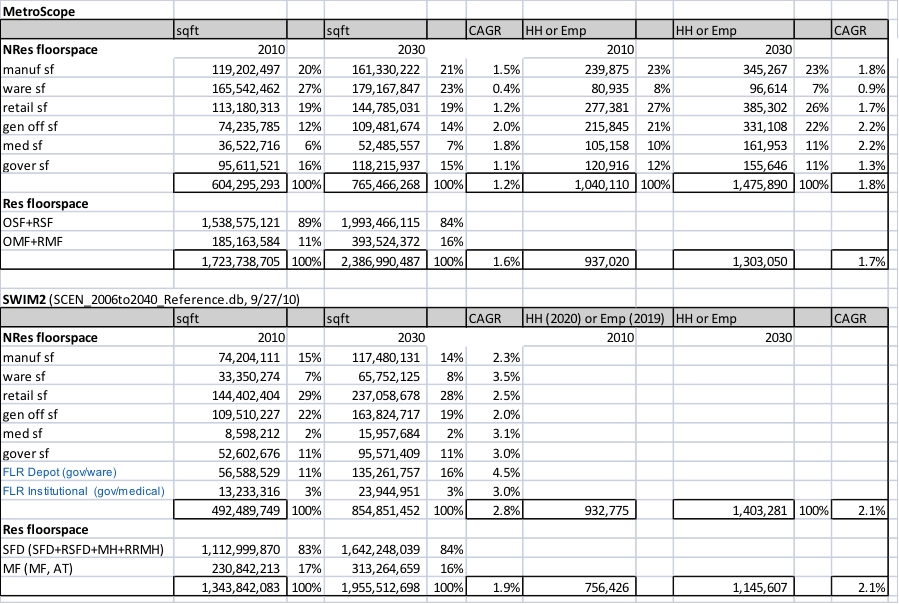
\includegraphics[width=6.5in]{ald/metroscope-comparison}
\caption{Comparison of SWIM2 versus MetroScope forecast floorspace and employment}
\label{fig:metroscope-comparison}
\end{figure}

\section{S3 parameters}
During the initial ALD S3 calibration, the three calibration steps using evolutionary algorithms were repeated using activity quantities, floorspace occupancy and price data from the S2 calibrated PI module (subsequently replaced with AA module). The ALD and AA modules were then jointly run through time to determine how well the behavior of each is affecting the other. The most important behavior of ALD with respect to the rest of the model system was that it provides an appropriate amount of increase in floorspace supply in zones where the rest of the system indicates that floorspace demand is high and little increase (or even a slight decrease) in floorspace supply in zones where the rest of the system indicates that floorspace demand is low. This appropriate response of development meeting demand was observed in initial sensitivity testing, with reasonable floorspace price increases.

The local signal for the demand for floorspace is the price of that floorspace that emerged from the PI module after PI accounts for changes in economic conditions and accessibilities. The PI module was calibrated in S2 calibration to match floorspace price distributions. In that initial S3 process no further adjustments were deemed necessary in ALD price sensitivity parameters $\beta_{4f}$ and $\beta_{6f}$ to ensure that over several years ALD responded with increased or decreased supply before prices reach unreasonable levels, particularly in zones where development capacity remains. It was noted that should the modelwide average prices or vacancy rates change unreasonably over time, $\beta_{2f}$ and $ASC_f$ parameters could also be adjusted. 

With the replacement of PI with AA and newer economic and demographic data (IMPLAN, Census), ALD may need to be tested and re-calibrated. S3 re-calibration required by recent adjustments to AA are currently on-going, and will likely need to continue to be evaluated over the life of this project.
